%   Filename    : chapter_4.tex

\chapter{Results and Discussion}

This chapter presents the performance of the proposed feature set and machine learning models for detecting PCR-induced chimeric reads in simulated mitochondrial Illumina data. The behaviour of the extracted features is first examined through descriptive and correlation analyses, followed by a comparison of baseline and tuned classifiers. The chapter then examines model performance in detail and investigates the contribution of individual features and feature families, including the impact of feature selection on classification performance.

The final dataset contained 31{,}986 reads for training and 7{,}997 reads for testing, with classes balanced (approximately 4{,}000 clean and 4{,}000 chimeric reads in the test split).

\section{Descriptive Analysis of Features}

\subsection{Summary Statistics Per Class}

Summary statistics were computed separately for clean reads (class~0) and chimeric reads (class~1) to characterize the distributional behavior of the features. For each feature, the mean, standard deviation, median, first and third quartiles (Q1, Q3), interquartile range (IQR), minimum, maximum, and sample size (\(n\)) were calculated.

Only a subset of the features is summarized in the main text to highlight key trends, and not all summary statistics columns are shown for brevity. The complete set of per-class summary statistics for all features is provided in Appendix~\ref{app:summary_stats} (Table~\ref{tab:feature_summary_full}).

\subsubsection{Alignment and Supplementary Alignment Features}

Features related to supplementary alignments show strong separation between classes. Chimeric reads frequently exhibit supplementary alignments, reflected by higher values of \texttt{has\_sa}, \texttt{sa\_count}, and \texttt{num\_segments}, whereas clean reads consistently show a single alignment segment with no supplementary mappings. Table~\ref{tab:key_feature_summary} shows that \texttt{has\_sa} is present in chimeric reads (mean = 0.406) but absent in clean reads (mean = 0.000), while \texttt{num\_segments} increases from a constant value of 1.000 in clean reads to a mean of 1.406 in chimeric reads. These patterns align with the expected structure of chimeric reads and indicate that alignment-based features are highly informative.

\subsubsection{Clipping-Based Features}

Clipping-related features, including \texttt{softclip\_left}, \texttt{softclip\_right}, and \texttt{total\_clipped\_bases}, display higher values and broader distributions in chimeric reads. In chimeric reads, \texttt{total\_clipped\_bases} reaches 25.44 on average, with a median of 19.0 and an IQR of 48.0, while \texttt{softclip\_left} and \texttt{softclip\_right} have averages of 12.55 and 12.90, medians of 0.0, and IQRs of 19.0. Clean reads maintain values near zero across all these metrics. These patterns indicate substantial clipping and increased variability in chimeric reads, reflecting junction-like alignment fragmentation, whereas clean reads remain unaltered.

\subsubsection{K-mer Distribution Features}

K-mer--based features, including \texttt{kmer\_js\_divergence} and \texttt{kmer\_cosine\_diff}, show only minor differences between clean and chimeric reads. In chimeric reads, \texttt{kmer\_js\_divergence} has a mean of 0.974 with a median of 0.986, and \texttt{kmer\_cosine\_diff} has a mean of 0.974 with a median of 0.986. Clean reads show similar values, with \texttt{kmer\_js\_divergence} at 0.976 with a median of 0.986, and \texttt{kmer\_cosine\_diff} at 0.976 with a median of 0.986. The close similarity of the means, medians, and overall ranges of values indicates that these features alone provide limited ability to distinguish clean from chimeric reads.

\subsubsection{Microhomology Features}

Microhomology-related features, including \texttt{microhomology\_length} and \texttt{microhomology\_gc}, exhibit nearly identical summary statistics between clean and chimeric reads. Most reads in both classes have short or zero-length microhomologies. Table~\ref{tab:key_feature_summary} shows that \texttt{microhomology\_gc} has a mean of 0.172 and a median of 0.0 in both clean and chimeric reads, while \texttt{microhomology\_length} averages 0.458 with a median of 0.0 in chimeric reads and 0.462 with a median of 0.0 in clean reads. These values indicate that microhomology features alone provide limited discriminatory power and are more appropriately considered as supporting evidence.

The summary statistics indicate that alignment-based and clipping-based features provide the strongest class separation, k-mer features contribute limited but complementary signal, and microhomology features exhibit minimal discriminative power on their own. These observations motivate the combined multi-feature approach used in subsequent modeling and evaluation.

\begin{table}[H]
\centering
\caption{Summary statistics of selected key features by class.}
\label{tab:key_feature_summary}
\begin{tabular}{llrrrr}
\toprule
Feature & Class & Mean & Std & Median & IQR \\
\midrule
has\_sa & chimeric & 0.406 & 0.491 & 0.0 & 1.0 \\
has\_sa & clean    & 0.000 & 0.000 & 0.0 & 0.0 \\

num\_segments & chimeric & 1.406 & 0.491 & 1.0 & 1.0 \\
num\_segments & clean    & 1.000 & 0.000 & 1.0 & 0.0 \\

softclip\_left & chimeric & 12.55 & 21.90 & 0.0 & 19.0 \\
softclip\_left & clean    & 0.23  & 1.54  & 0.0 & 0.0  \\

softclip\_right & chimeric & 12.90 & 22.12 & 0.0 & 19.0 \\
softclip\_right & clean    & 0.21  & 1.51  & 0.0 & 0.0  \\

total\_clipped\_bases & chimeric & 25.44 & 25.48 & 19.0 & 48.0 \\
total\_clipped\_bases & clean    & 0.44  & 2.16  & 0.0  & 0.0  \\

kmer\_js\_divergence & chimeric & 0.974 & 0.025 & 0.986 & 0.043 \\
kmer\_js\_divergence & clean    & 0.976 & 0.025 & 0.986 & 0.040 \\

kmer\_cosine\_diff & chimeric & 0.974 & 0.026 & 0.986 & 0.042 \\
kmer\_cosine\_diff & clean    & 0.976 & 0.025 & 0.986 & 0.041 \\

microhomology\_length & chimeric & 0.458 & 0.755 & 0.0 & 1.0 \\
microhomology\_length & clean    & 0.462 & 0.758 & 0.0 & 1.0 \\

microhomology\_gc  & chimeric & 0.172 & 0.361 & 0.0 & 0.0 \\
microhomology\_gc  & clean    & 0.172 & 0.361 & 0.0 & 0.0 \\
\bottomrule
\end{tabular}
\end{table}

Boxplots were generated for each feature, with the x-axis representing the class (clean reads and chimeric reads) and the y-axis representing the feature value. Figure~\ref{fig:boxplots_all_features} presents a panel of selected key features, while boxplots for all numeric features are provided in Appendix~\ref{app:boxplots_by_family}.

For clipping-related features (\texttt{softclip\_left}, \texttt{softclip\_right}, and \texttt{total\_clipped\_bases}), chimeric reads exhibit higher medians and longer upper whiskers than clean reads, indicating increased variability and the presence of split alignments.

Supplementary alignment features (\texttt{has\_sa} and \texttt{sa\_count}) show that clean reads are largely zero, whereas chimeric reads display a wider distribution, reflecting frequent supplementary alignments.

K-mer metrics (\texttt{kmer\_js\_divergence} and \texttt{kmer\_cosine\_diff}) show a slight upward shift for chimeric reads, but substantial overlap with clean reads indicates low discriminative power.

Microhomology features (\texttt{microhomology\_length} and \texttt{microhomology\_gc}) have nearly overlapping distributions for both classes, consistent with their low standalone predictive importance.

\begin{figure}[H]
\centering

\begin{subfigure}[b]{0.32\textwidth}
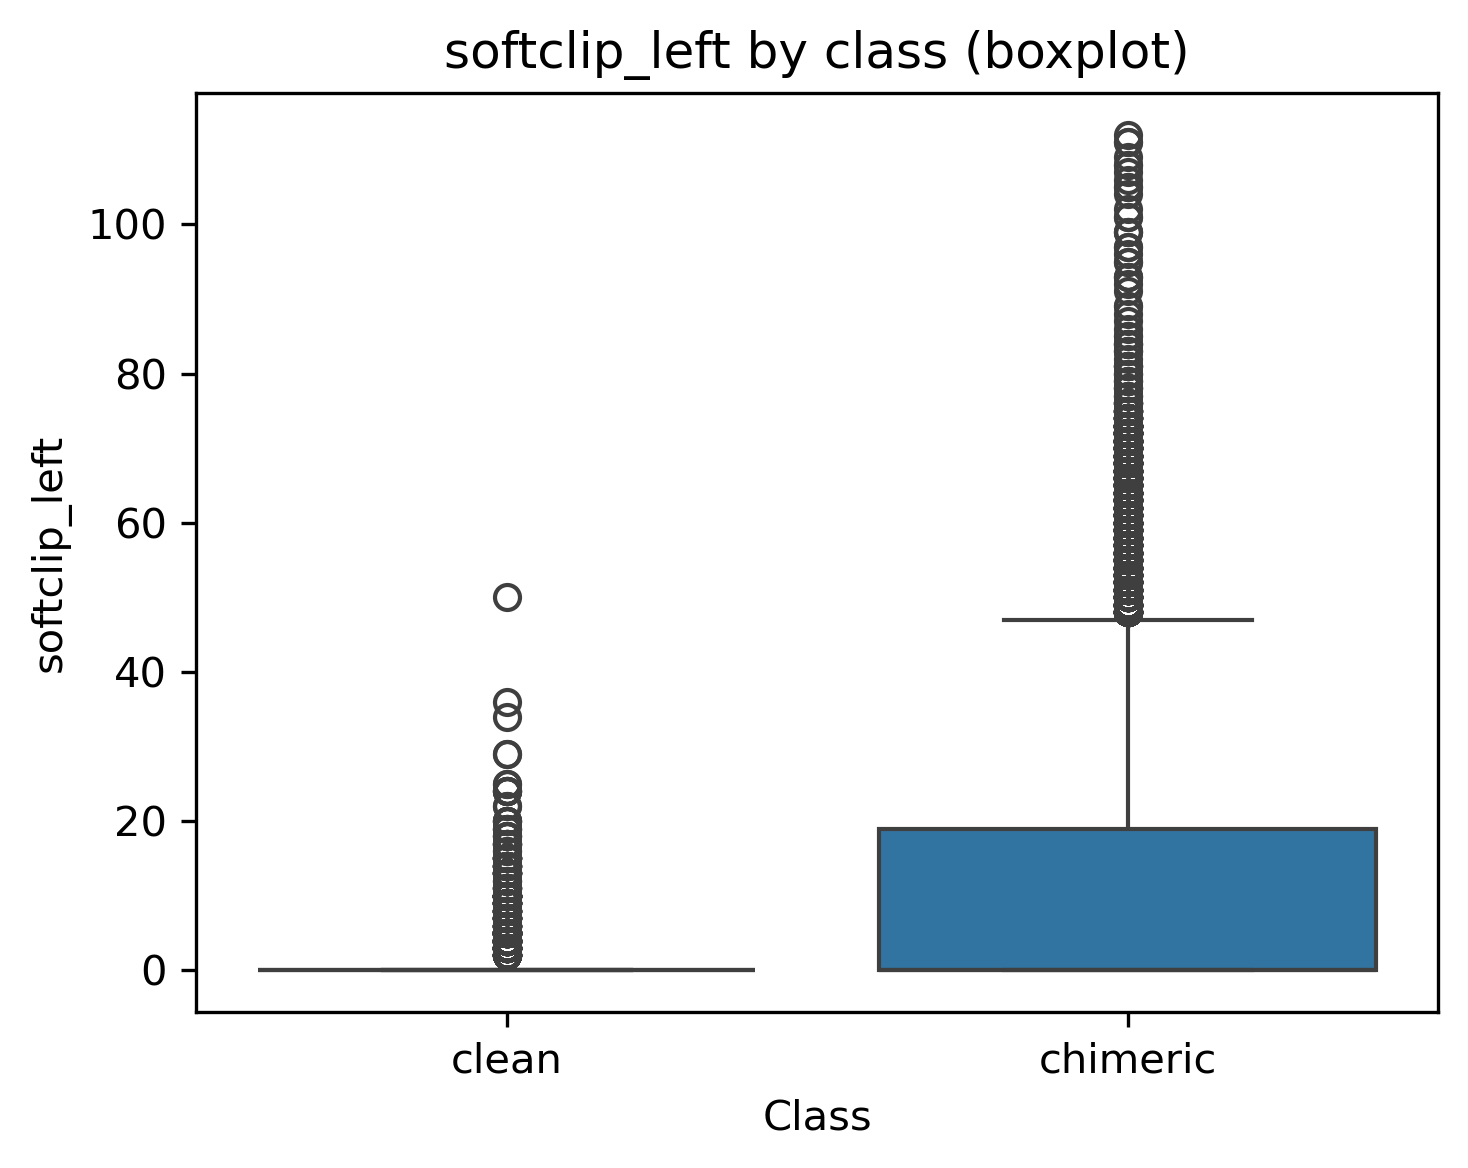
\includegraphics[width=\textwidth]{../notebooks/figures/boxplots/box_softclip_left.png}
\caption{Softclip left}
\label{fig:box_softclip_left}
\end{subfigure}
\hfill
\begin{subfigure}[b]{0.32\textwidth}
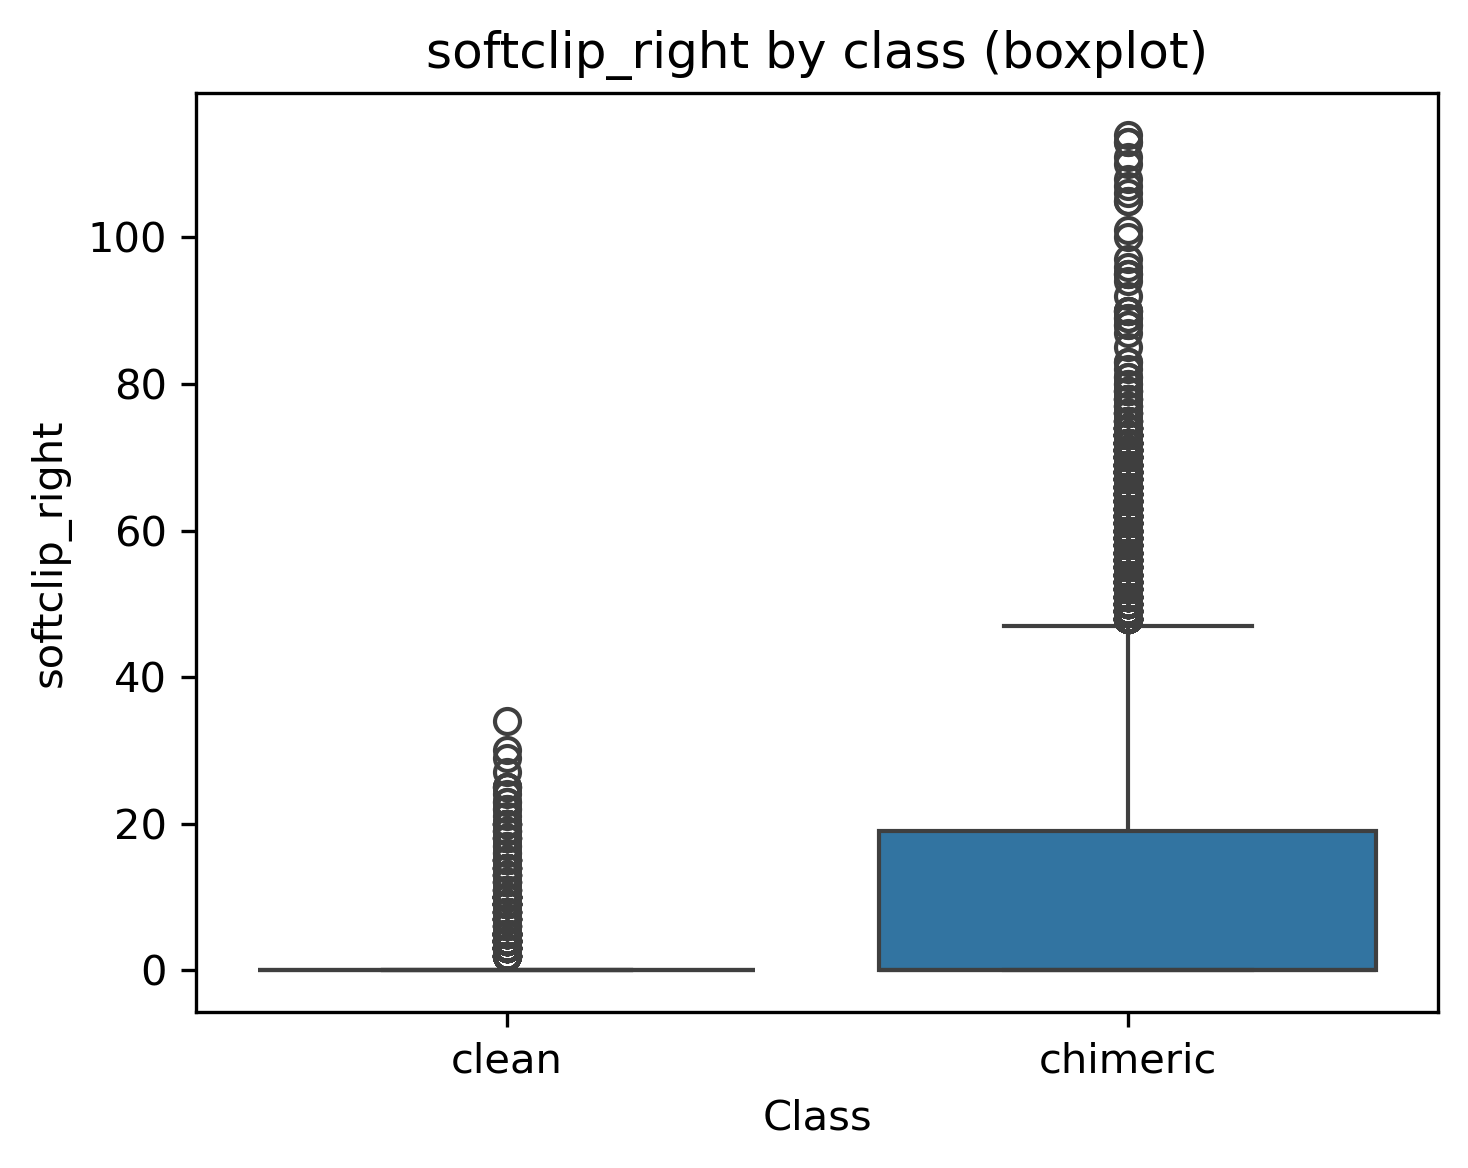
\includegraphics[width=\textwidth]{../notebooks/figures/boxplots/box_softclip_right.png}
\caption{Softclip right}
\label{fig:box_softclip_right}
\end{subfigure}
\hfill
\begin{subfigure}[b]{0.32\textwidth}
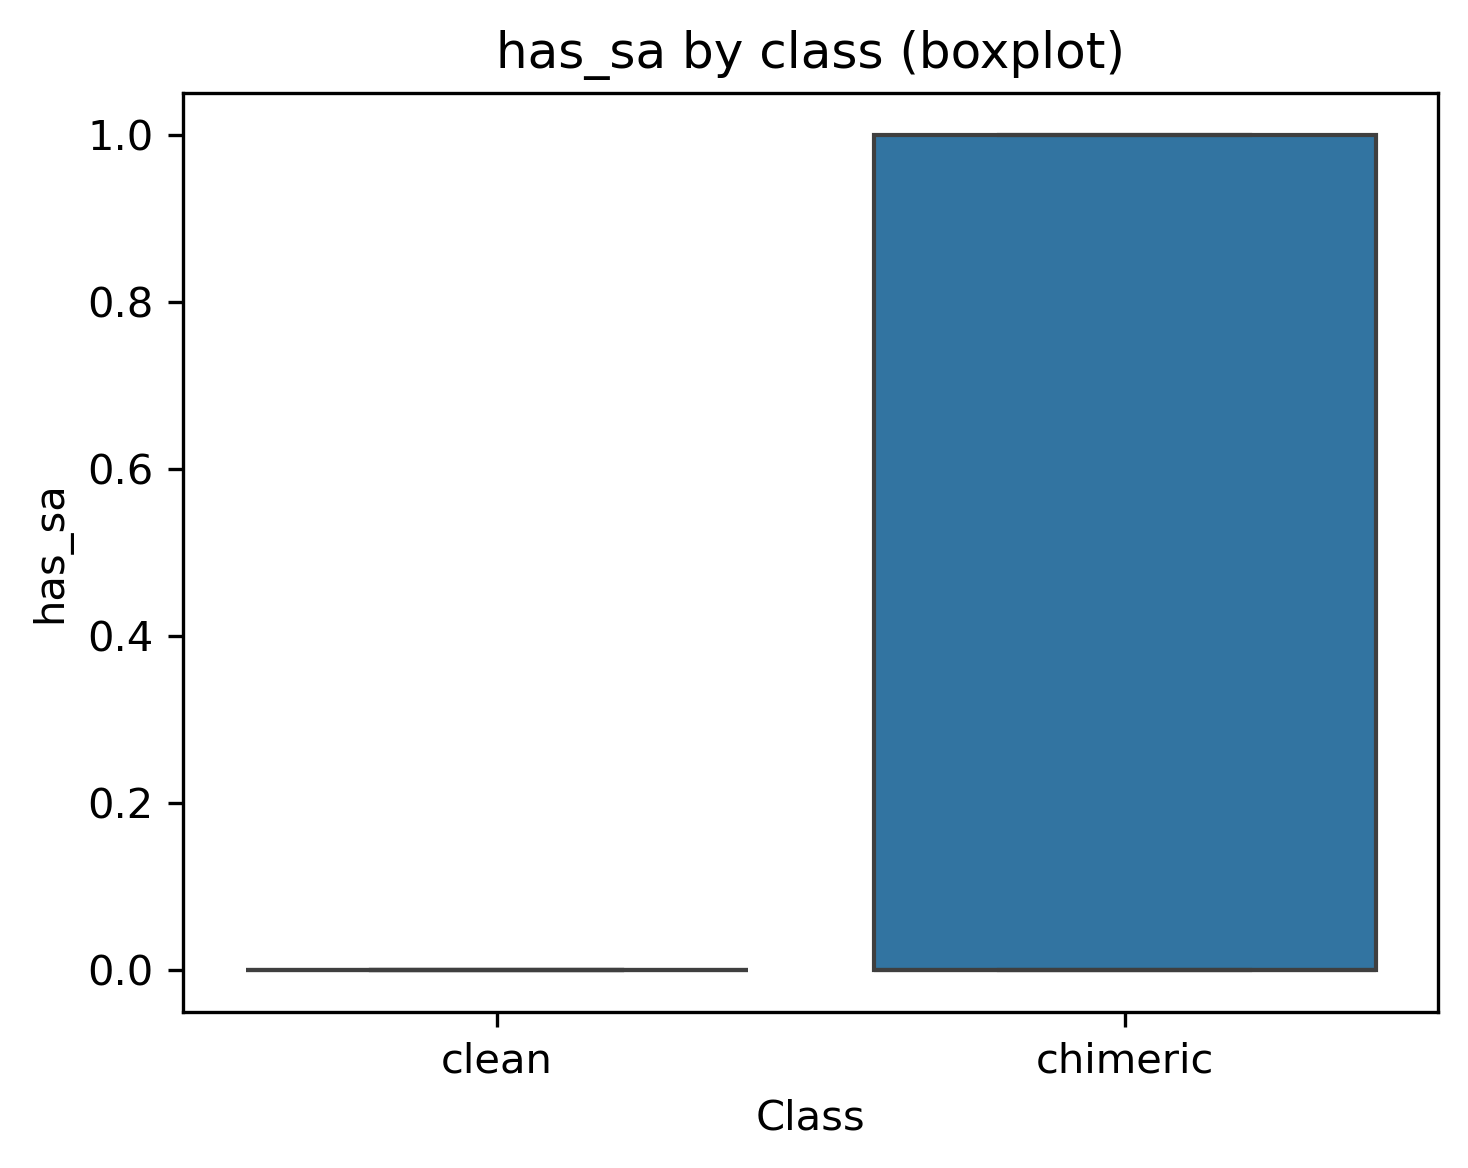
\includegraphics[width=\textwidth]{../notebooks/figures/boxplots/box_has_sa.png}
\caption{Has SA}
\label{fig:box_has_sa}
\end{subfigure}

\vspace{0.5em}

\begin{subfigure}[b]{0.32\textwidth}
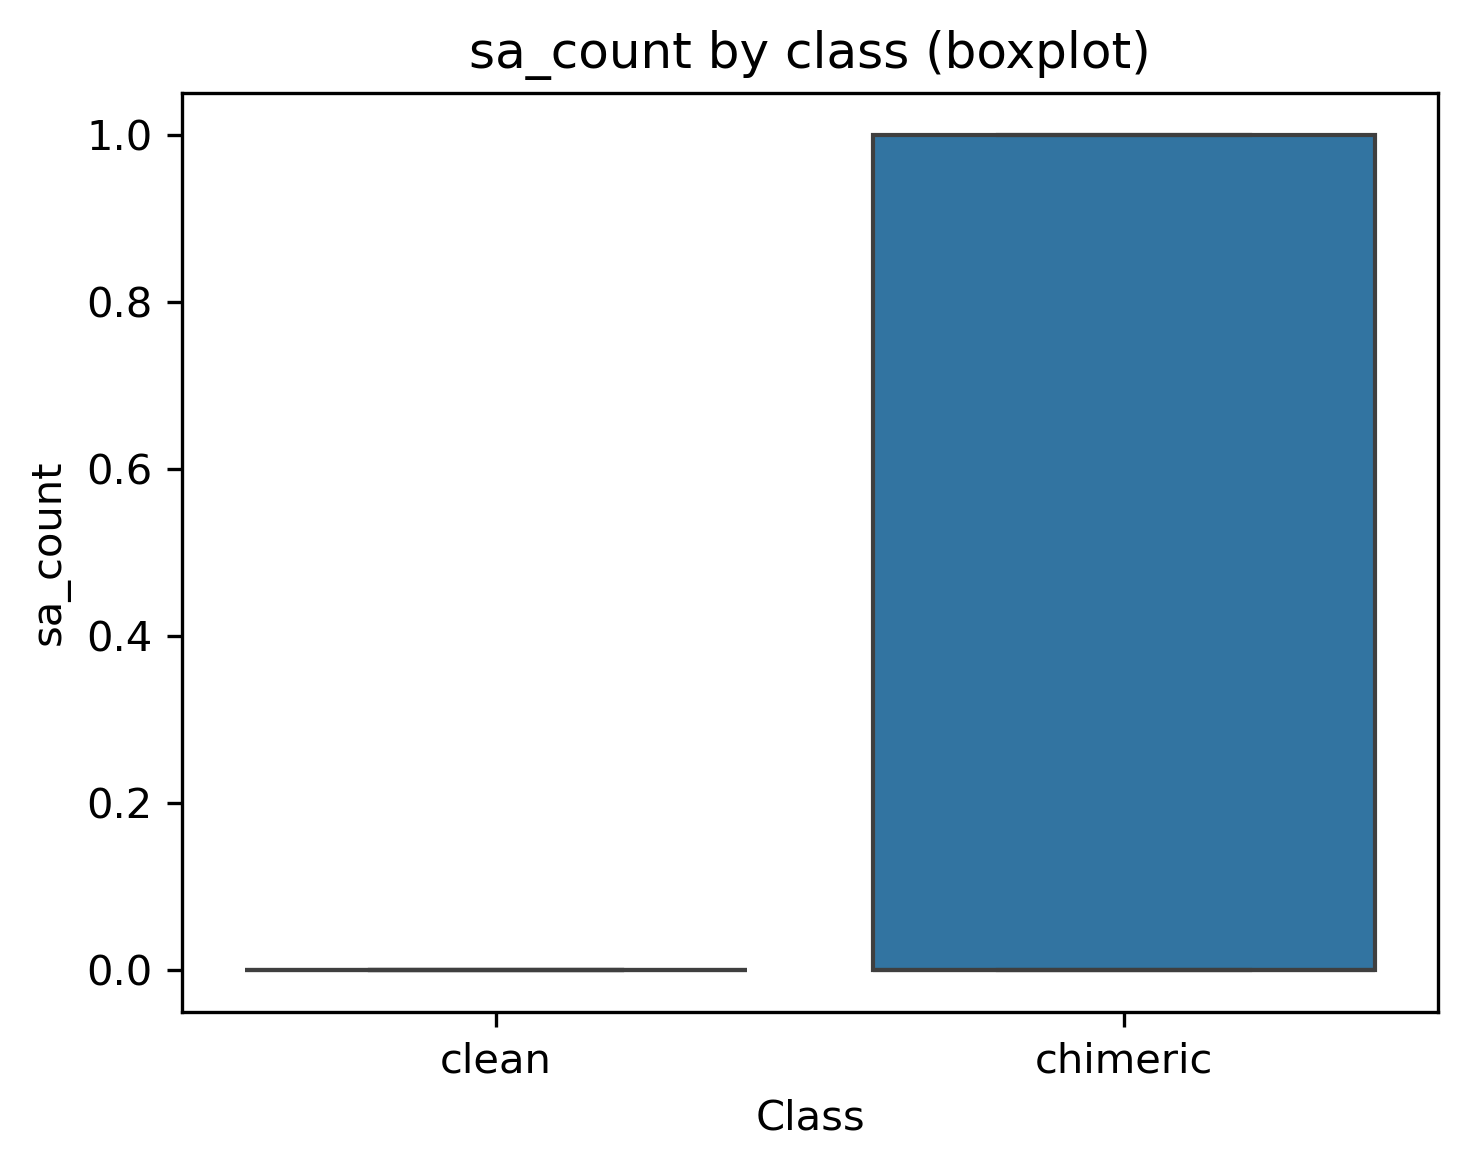
\includegraphics[width=\textwidth]{../notebooks/figures/boxplots/box_sa_count.png}
\caption{SA count}
\label{fig:box_sa_count}
\end{subfigure}
\hfill
\begin{subfigure}[b]{0.32\textwidth}
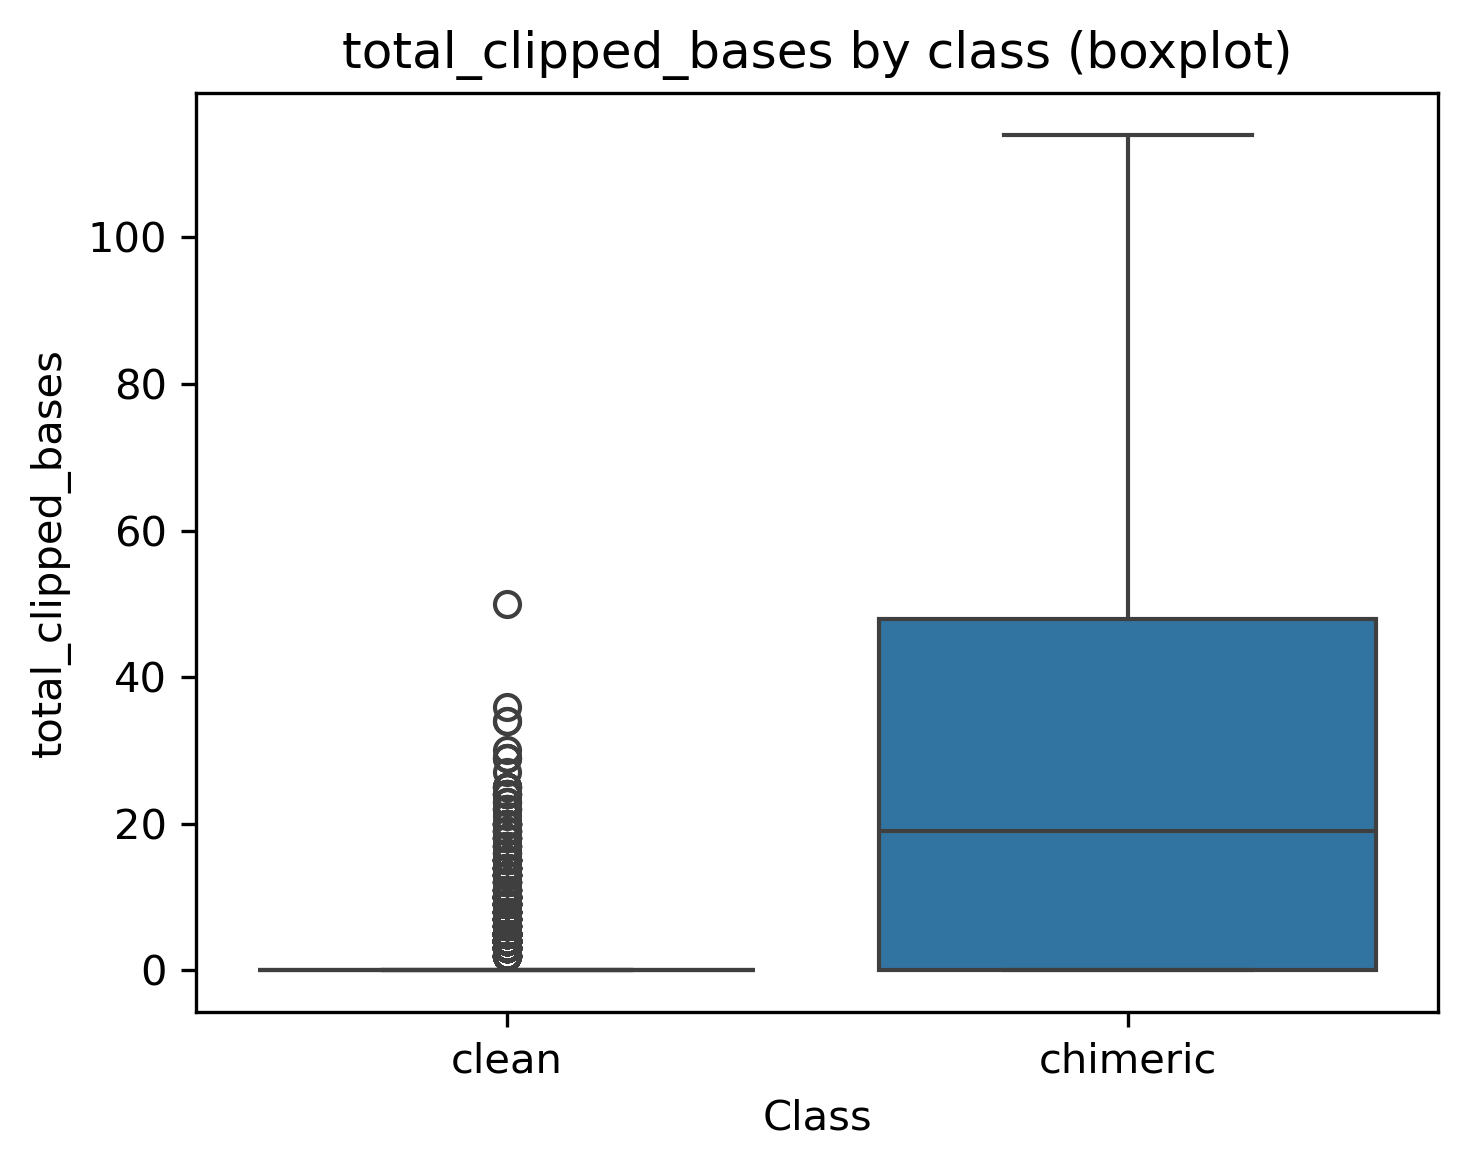
\includegraphics[width=\textwidth]{../notebooks/figures/boxplots/box_total_clipped_bases.png}
\caption{Total clipped bases}
\label{fig:box_total_clipped_bases}
\end{subfigure}
\hfill
\begin{subfigure}[b]{0.32\textwidth}
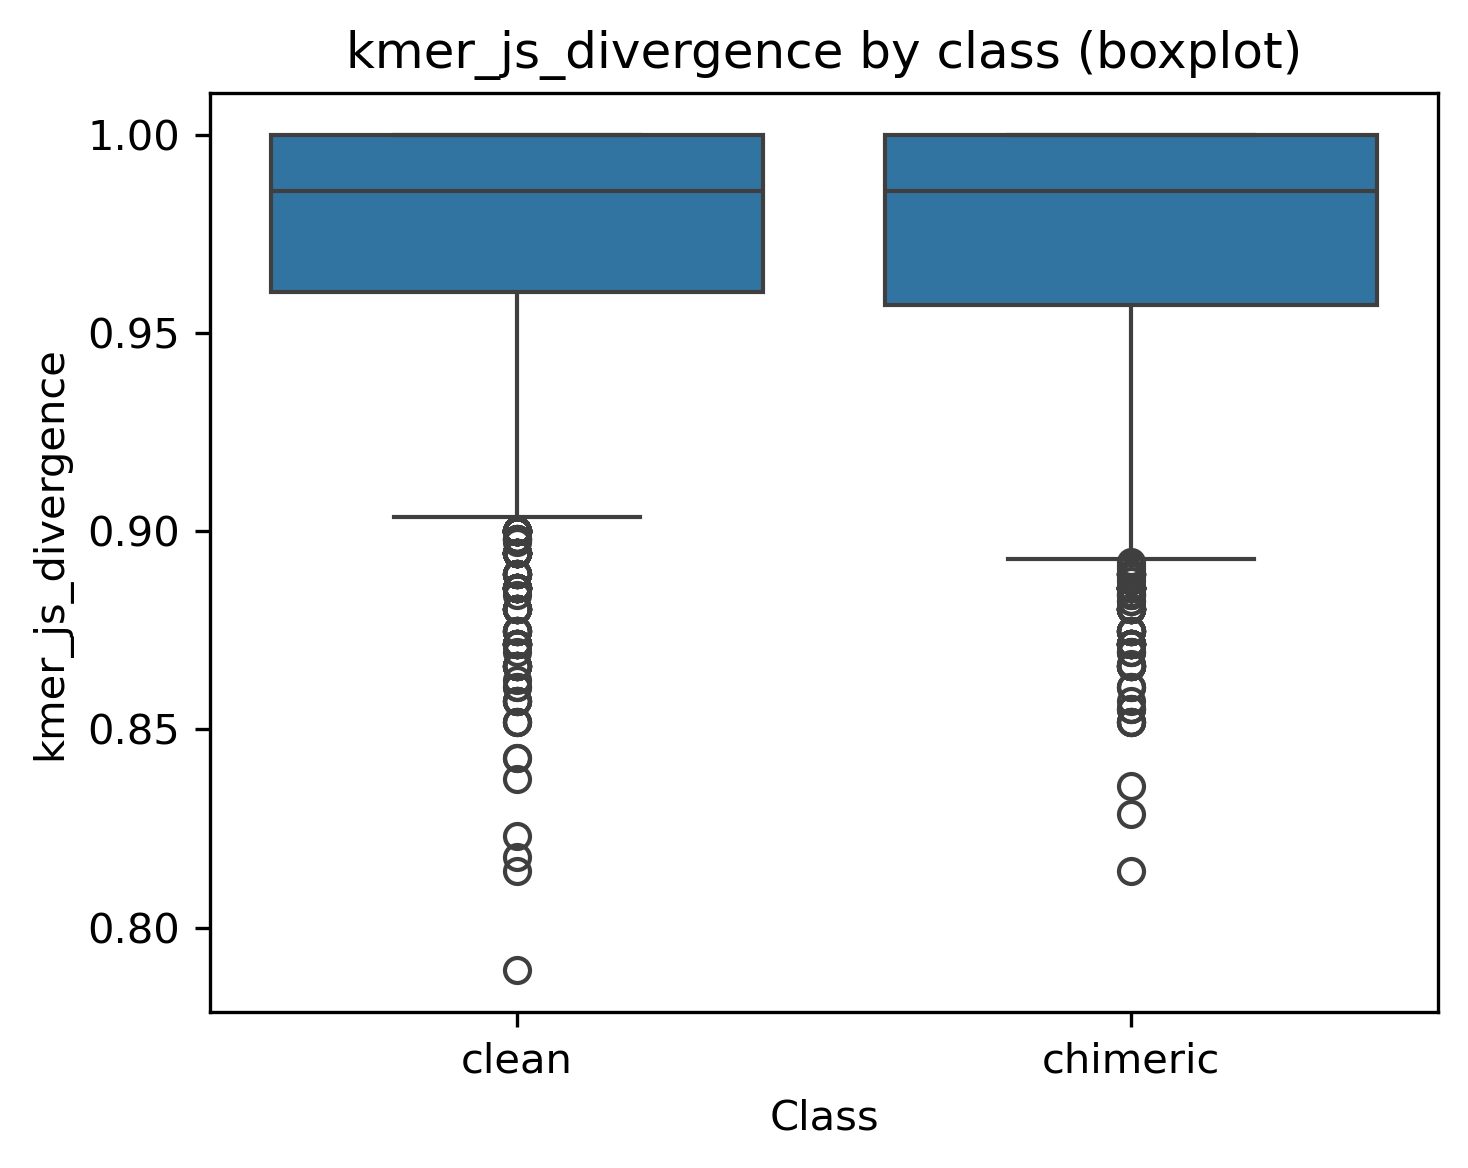
\includegraphics[width=\textwidth]{../notebooks/figures/boxplots/box_kmer_js_divergence.png}
\caption{K-mer JS divergence}
\label{fig:box_kmer_js_divergence}
\end{subfigure}

\vspace{0.5em}

\begin{subfigure}[b]{0.32\textwidth}
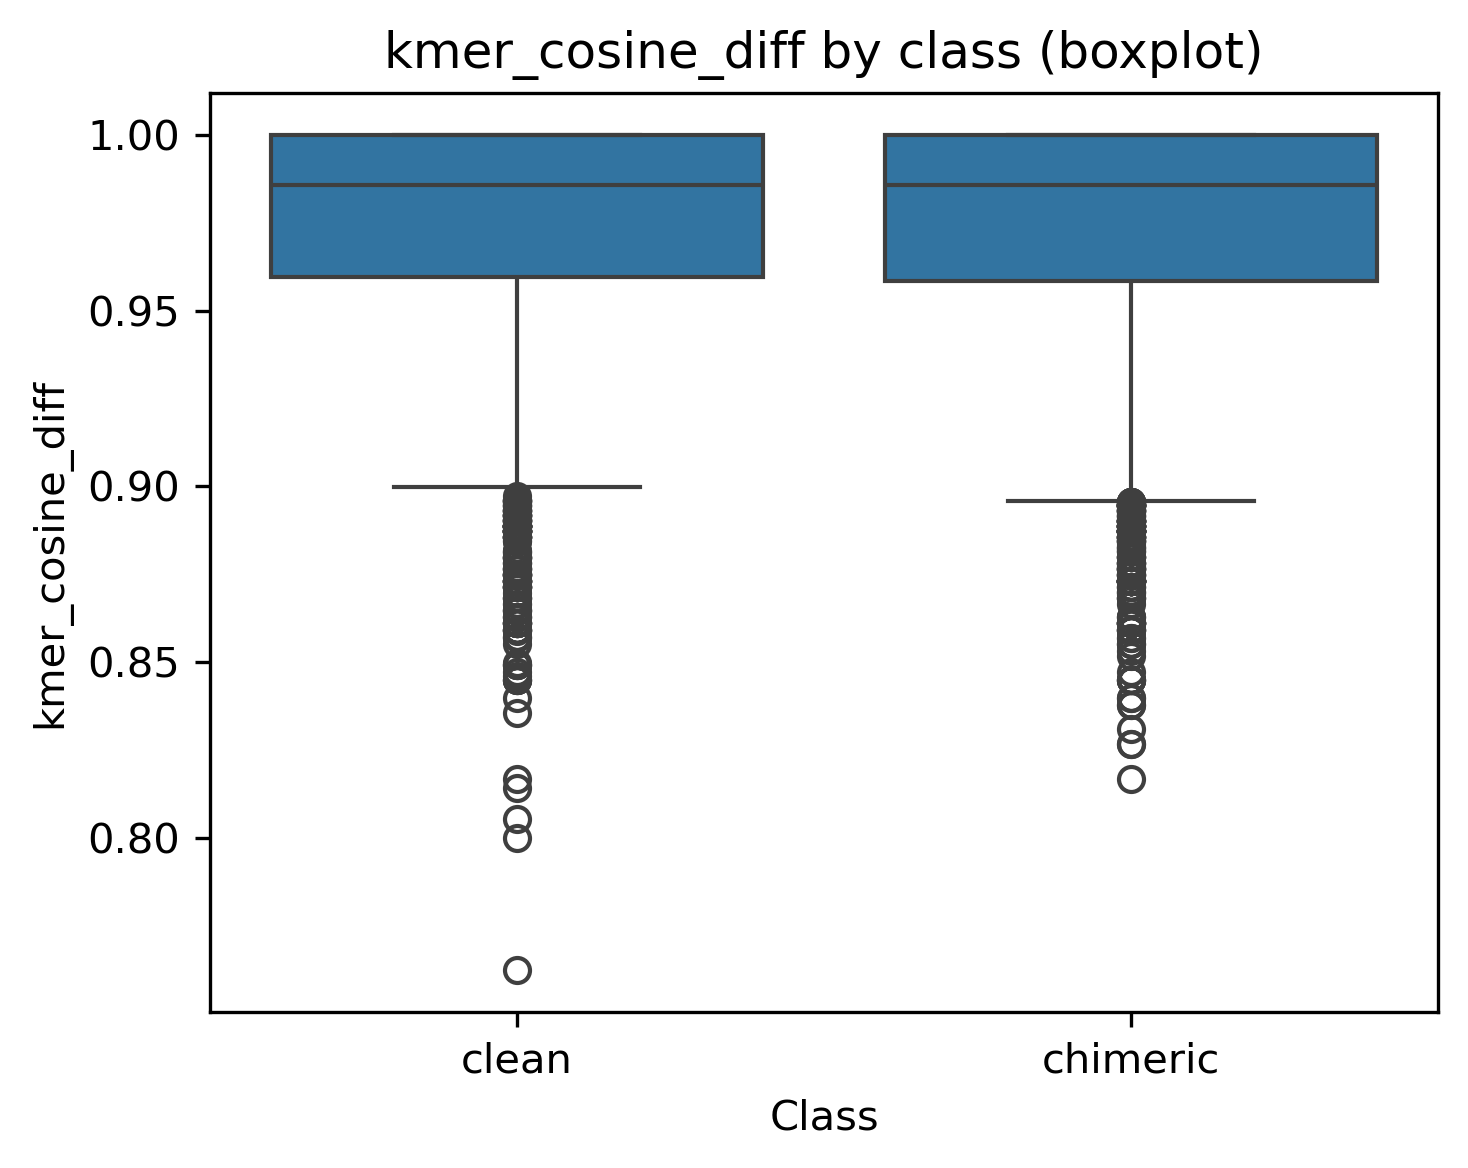
\includegraphics[width=\textwidth]{../notebooks/figures/boxplots/box_kmer_cosine_diff.png}
\caption{K-mer cosine difference}
\label{fig:box_kmer_cosine_diff}
\end{subfigure}
\hfill
\begin{subfigure}[b]{0.32\textwidth}
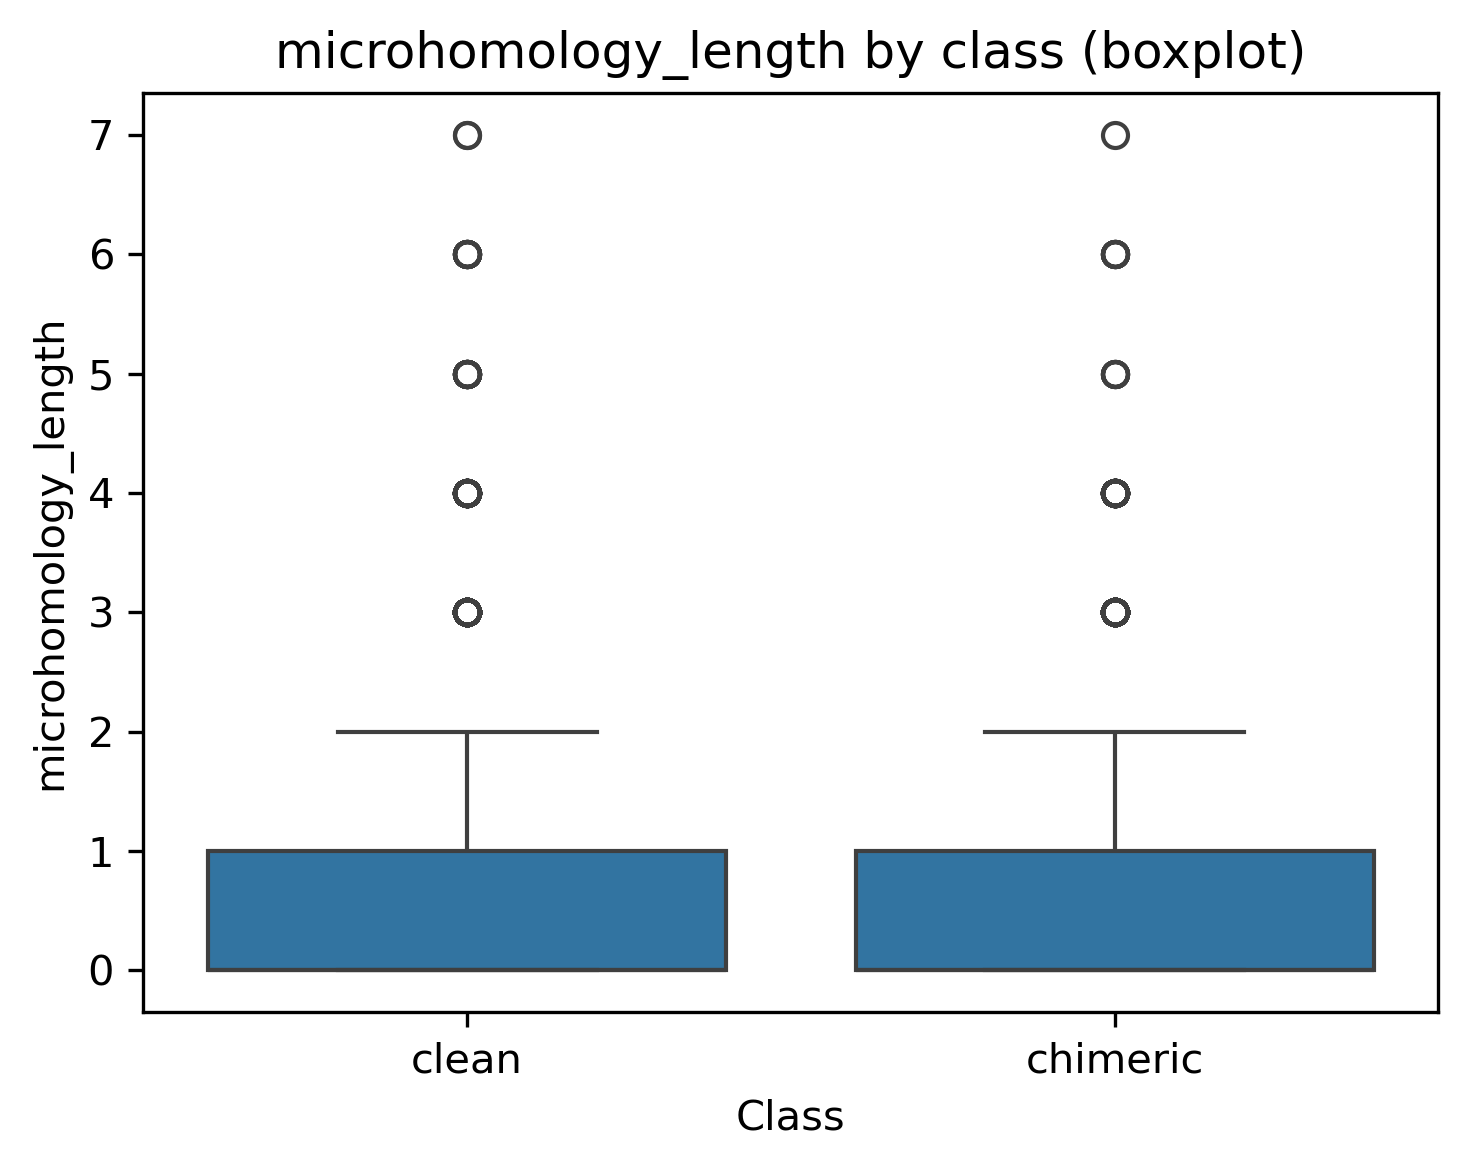
\includegraphics[width=\textwidth]{../notebooks/figures/boxplots/box_microhomology_length.png}
\caption{Microhomology length}
\label{fig:box_microhomology_length}
\end{subfigure}
\hfill
\begin{subfigure}[b]{0.32\textwidth}
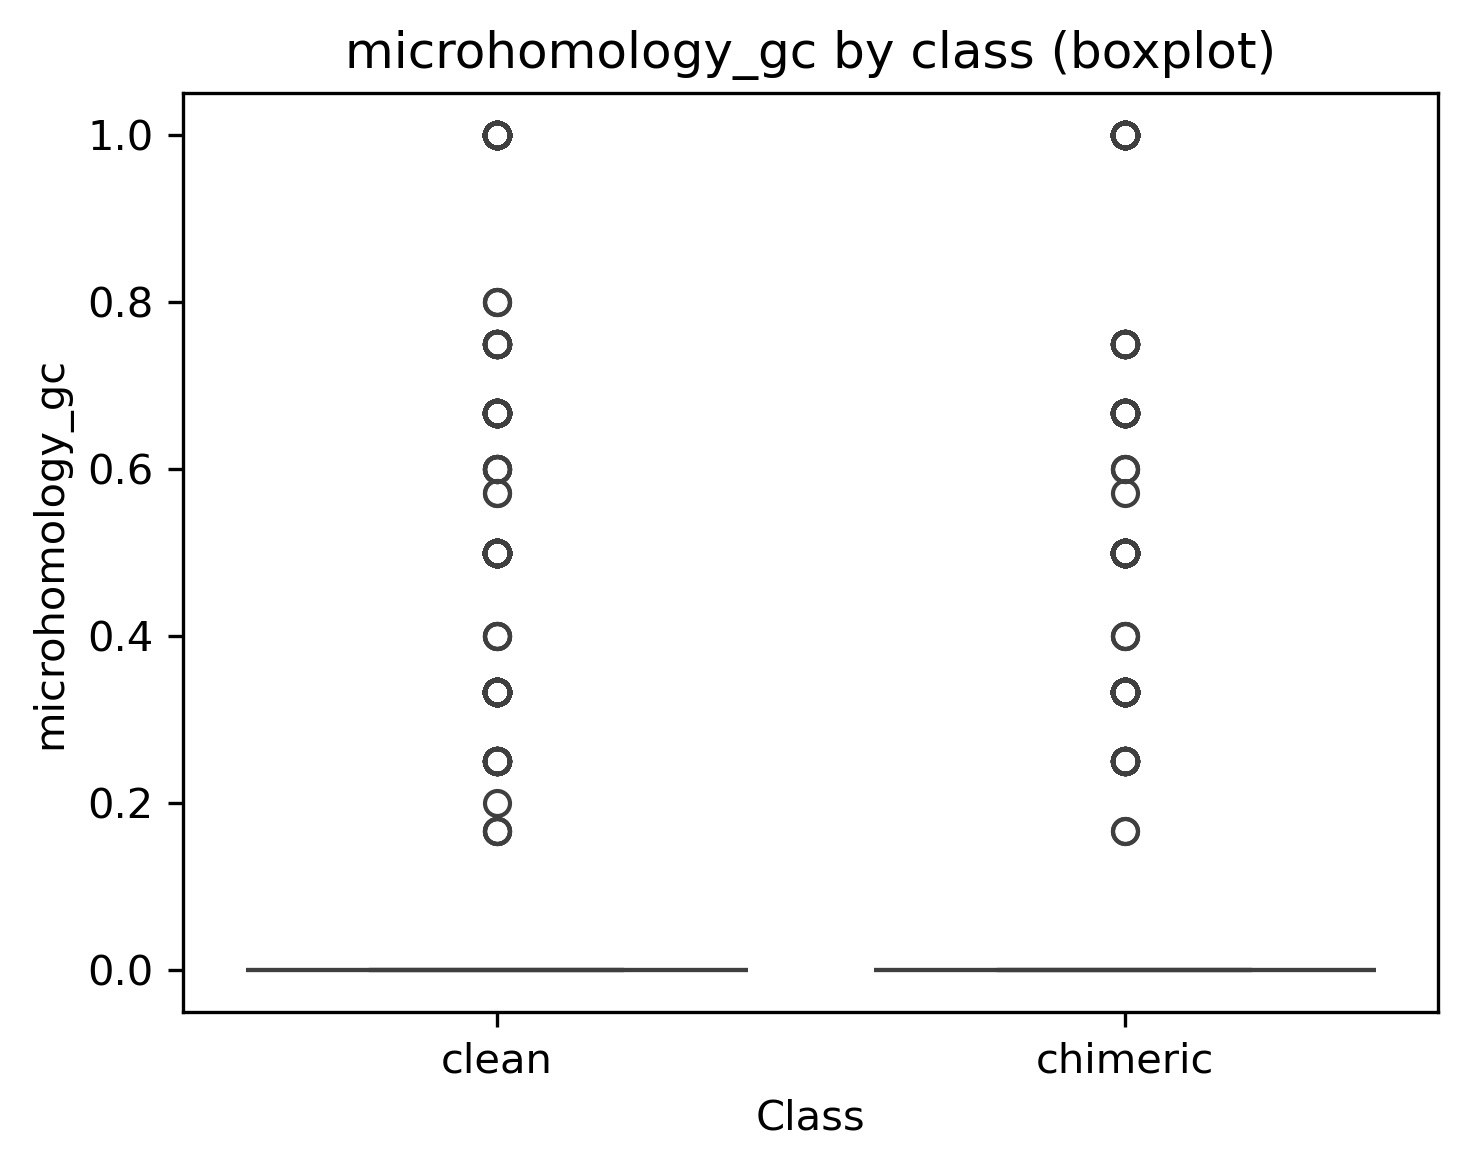
\includegraphics[width=\textwidth]{../notebooks/figures/boxplots/box_microhomology_gc.png}
\caption{Microhomology GC}
\label{fig:box_microhomology_gc}
\end{subfigure}

\caption{Boxplots of selected features for clean and chimeric reads.}
\label{fig:boxplots_all_features}
\end{figure}

\subsection{Correlation Analysis of Extracted Features}

A feature correlation heatmap (Figure~\ref{fig:correlation_heatmap}) was generated to examine relationships among the extracted variables and to identify patterns of redundancy and independence within the feature set. The analysis shows that alignment-related and clipping-related features form a strongly correlated cluster, including indicators of supplementary alignments, alignment segment counts, positional differences, and soft-clipping measures. These features capture related aspects of alignment fragmentation, which is a known characteristic of chimeric reads, and several show moderate correlations with the class label, supporting their relevance for distinguishing chimeric from clean reads. In contrast, general read-quality and alignment-quality metrics, such as read length, base quality, and mapping quality, exhibit weak correlations with most split-alignment features, indicating that they provide distinct information rather than overlapping with alignment-derived signals. Sequence-based features display a similar pattern of independence, as k-mer divergence metrics show weak correlations with other feature groups, while microhomology features exhibit generally low correlations with both alignment-based and k-mer-based features. Overall, the correlation structure highlights intentional redundancy within alignment-derived features and clear separation between feature families, supporting the use of features that capture different aspects of chimeric read characteristics to improve chimera classification.

\begin{figure}[H]
\centering
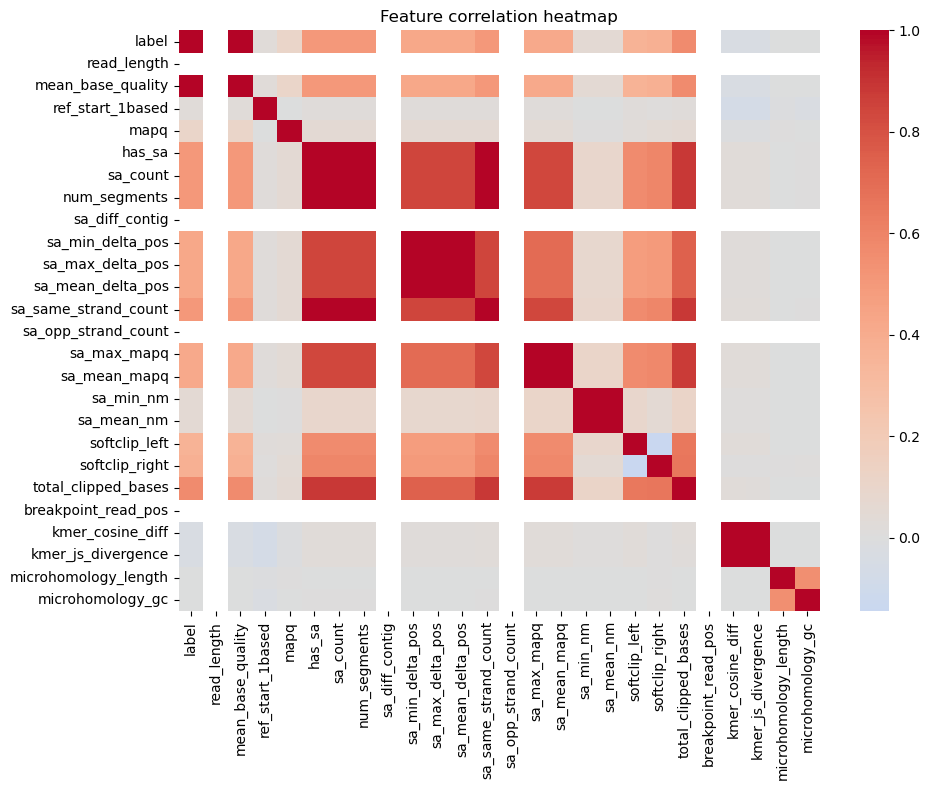
\includegraphics[width=0.75\textwidth]{../notebooks/figures/correlation.png}
\caption{Feature correlation heatmap showing relationships among alignment-derived and sequence-derived features.}
\label{fig:correlation_heatmap}
\end{figure}

\section{Baseline Classification Performance}

Table~\ref{tab:baseline_models_noq} summarises the performance of thirteen baseline classifiers trained on the engineered feature set and evaluated on a held-out test set. All models were trained using default hyperparameters, without dedicated tuning.

The dummy baseline, which always predicts the same class regardless of the input features, achieved a test accuracy of approximately 0.50 and an F1-score of 0.67. This reflects the balanced class distribution and serves as a lower bound for meaningful model performance.

Across the remaining models, test F1-scores clustered within a narrow range, from approximately 0.75 to 0.78, with ROC--AUC values between about 0.82 and 0.85. Ensemble methods, including gradient boosting, CatBoost, LightGBM, XGBoost, bagging trees, and random forest, exhibited very similar performance. Among these, CatBoost and gradient boosting achieved the highest scores, with test F1-scores of approximately 0.775 and ROC--AUC values of approximately 0.84. Linear models, namely logistic regression and the calibrated linear SVM, performed slightly worse, with test F1-scores around 0.75. In contrast, Gaussian Naive Bayes lagged behind with a substantially lower F1-score of approximately 0.66, despite exhibiting extremely high precision for the chimeric class.

\input{tables/baseline_models_noq}

\begin{figure}[H]
\centering
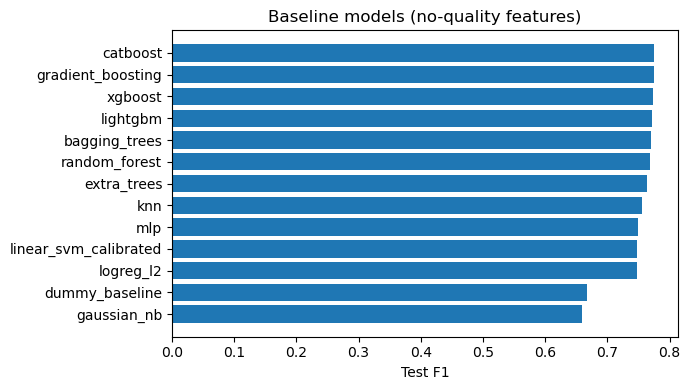
\includegraphics[width=0.8\linewidth]{figures/baseline_models_pair.png}
\caption{Test F1 of all baseline classifiers.}
\label{fig:baseline_f1}
\end{figure}

\section{Effect of Hyperparameter Tuning}

To assess whether performance could be improved further, ten model families underwent randomised hyperparameter search. The tuned metrics are summarised in Table~\ref{tab:tuned_models_noq}. Overall, tuning yielded modest but consistent gains for tree-based ensembles and boosting methods, while leaving linear models essentially unchanged or slightly worse.

CatBoost, gradient boosting, LightGBM, random forest, bagging trees, and extra trees experienced small increases in test F1 after tuning, typically on the order of \(\Delta \mathrm{F1} \approx 0.002\)--0.006, with corresponding improvements in ROC--AUC of up to approximately \(\Delta \mathrm{AUC} \approx 0.009\). In contrast, XGBoost and the multilayer perceptron showed negligible change or slight decreases in F1, while linear models did not benefit from tuning.

After tuning, gradient boosting achieved the best overall test performance, with a test F1-score of 0.776 and a ROC--AUC of 0.846. LightGBM and bagging trees followed closely, attaining test F1-scores of 0.774 and 0.772 and ROC--AUC values of 0.843 and 0.842, respectively. Random forest also improved modestly to a test F1-score of 0.772 with a ROC--AUC of 0.839. CatBoost, with a test F1-score of 0.775 and ROC--AUC of 0.843, achieved marginal changes relative to its baseline performance.

\input{tables/tuned_models_noq}

\begin{figure}[H]
\centering
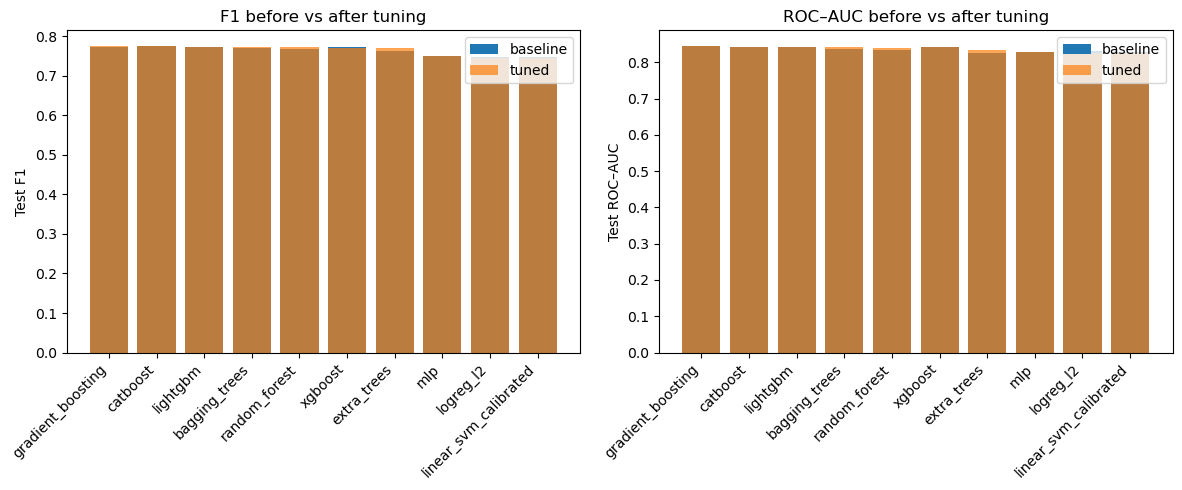
\includegraphics[width=\linewidth]{figures/f1_auc_tuning_pair.png}
\caption{Comparison of test F1 (left) and ROC--AUC (right) for baseline and tuned models.}
\label{fig:f1_auc_tuning}
\end{figure}

Because improvements are small and within cross-validation variability, tuning was interpreted as stabilising and slightly refining the models rather than completely altering their behaviour or their relative ranking.

\subsection{Confusion Matrix and Error Patterns}

Gradient Boosting was selected as the final classifier, as it demonstrated the best overall performance. Its classification report and confusion matrix show an overall accuracy of approximately 0.81, with a macro-averaged F1-score of about 0.80. For clean reads, the model achieved precision of 0.74 and recall of 0.96, while for chimeric reads it achieved precision of 0.94 and recall of 0.66, corresponding to an F1-score of 0.777 for the chimeric class.

Errors were asymmetric, with false negatives (chimeric reads predicted as clean) occurring more often than false positives. Specifically, the model misclassified 1{,}352 chimeric reads as clean and 181 clean reads as chimeric. This pattern indicates that the classifier is conservative, prioritising the avoidance of false chimera calls even if some true chimeric reads are missed. Consultation with PGC Visayas suggested that this conservative behaviour is generally acceptable, although further assessment is still needed to determine its downstream impact on analysis workflows.

\begin{figure}[H]
\centering

\includegraphics[width=0.5\linewidth]{figures/cm_pair_gradient_boosting.png}
\caption{Confusion matrix of the tuned Gradient Boosting classifier on the held-out test set.}
\label{fig:cm_gradient_boosting}
\end{figure}

\subsection{ROC and Precision--Recall Curves}

The receiver operating characteristic (ROC) and precision--recall (PR) curves further demonstrate the strong performance of the tuned Gradient Boosting classifier. The model achieved a ROC--AUC of approximately 0.84 and an average precision of approximately 0.88 on the held-out test set.

The PR curve shows that precision remains above 0.9 across a broad range of recall values up to roughly 0.5--0.6, after which precision gradually declines. This behaviour suggests that the classifier can assign very high confidence to a subset of chimeric reads, while the recovery of more ambiguous reads requires accepting lower precision. These curves indicate that Gradient Boosting provides a strong balance between sensitivity and specificity for the detection of chimeric reads.

\begin{figure}[H]
\centering
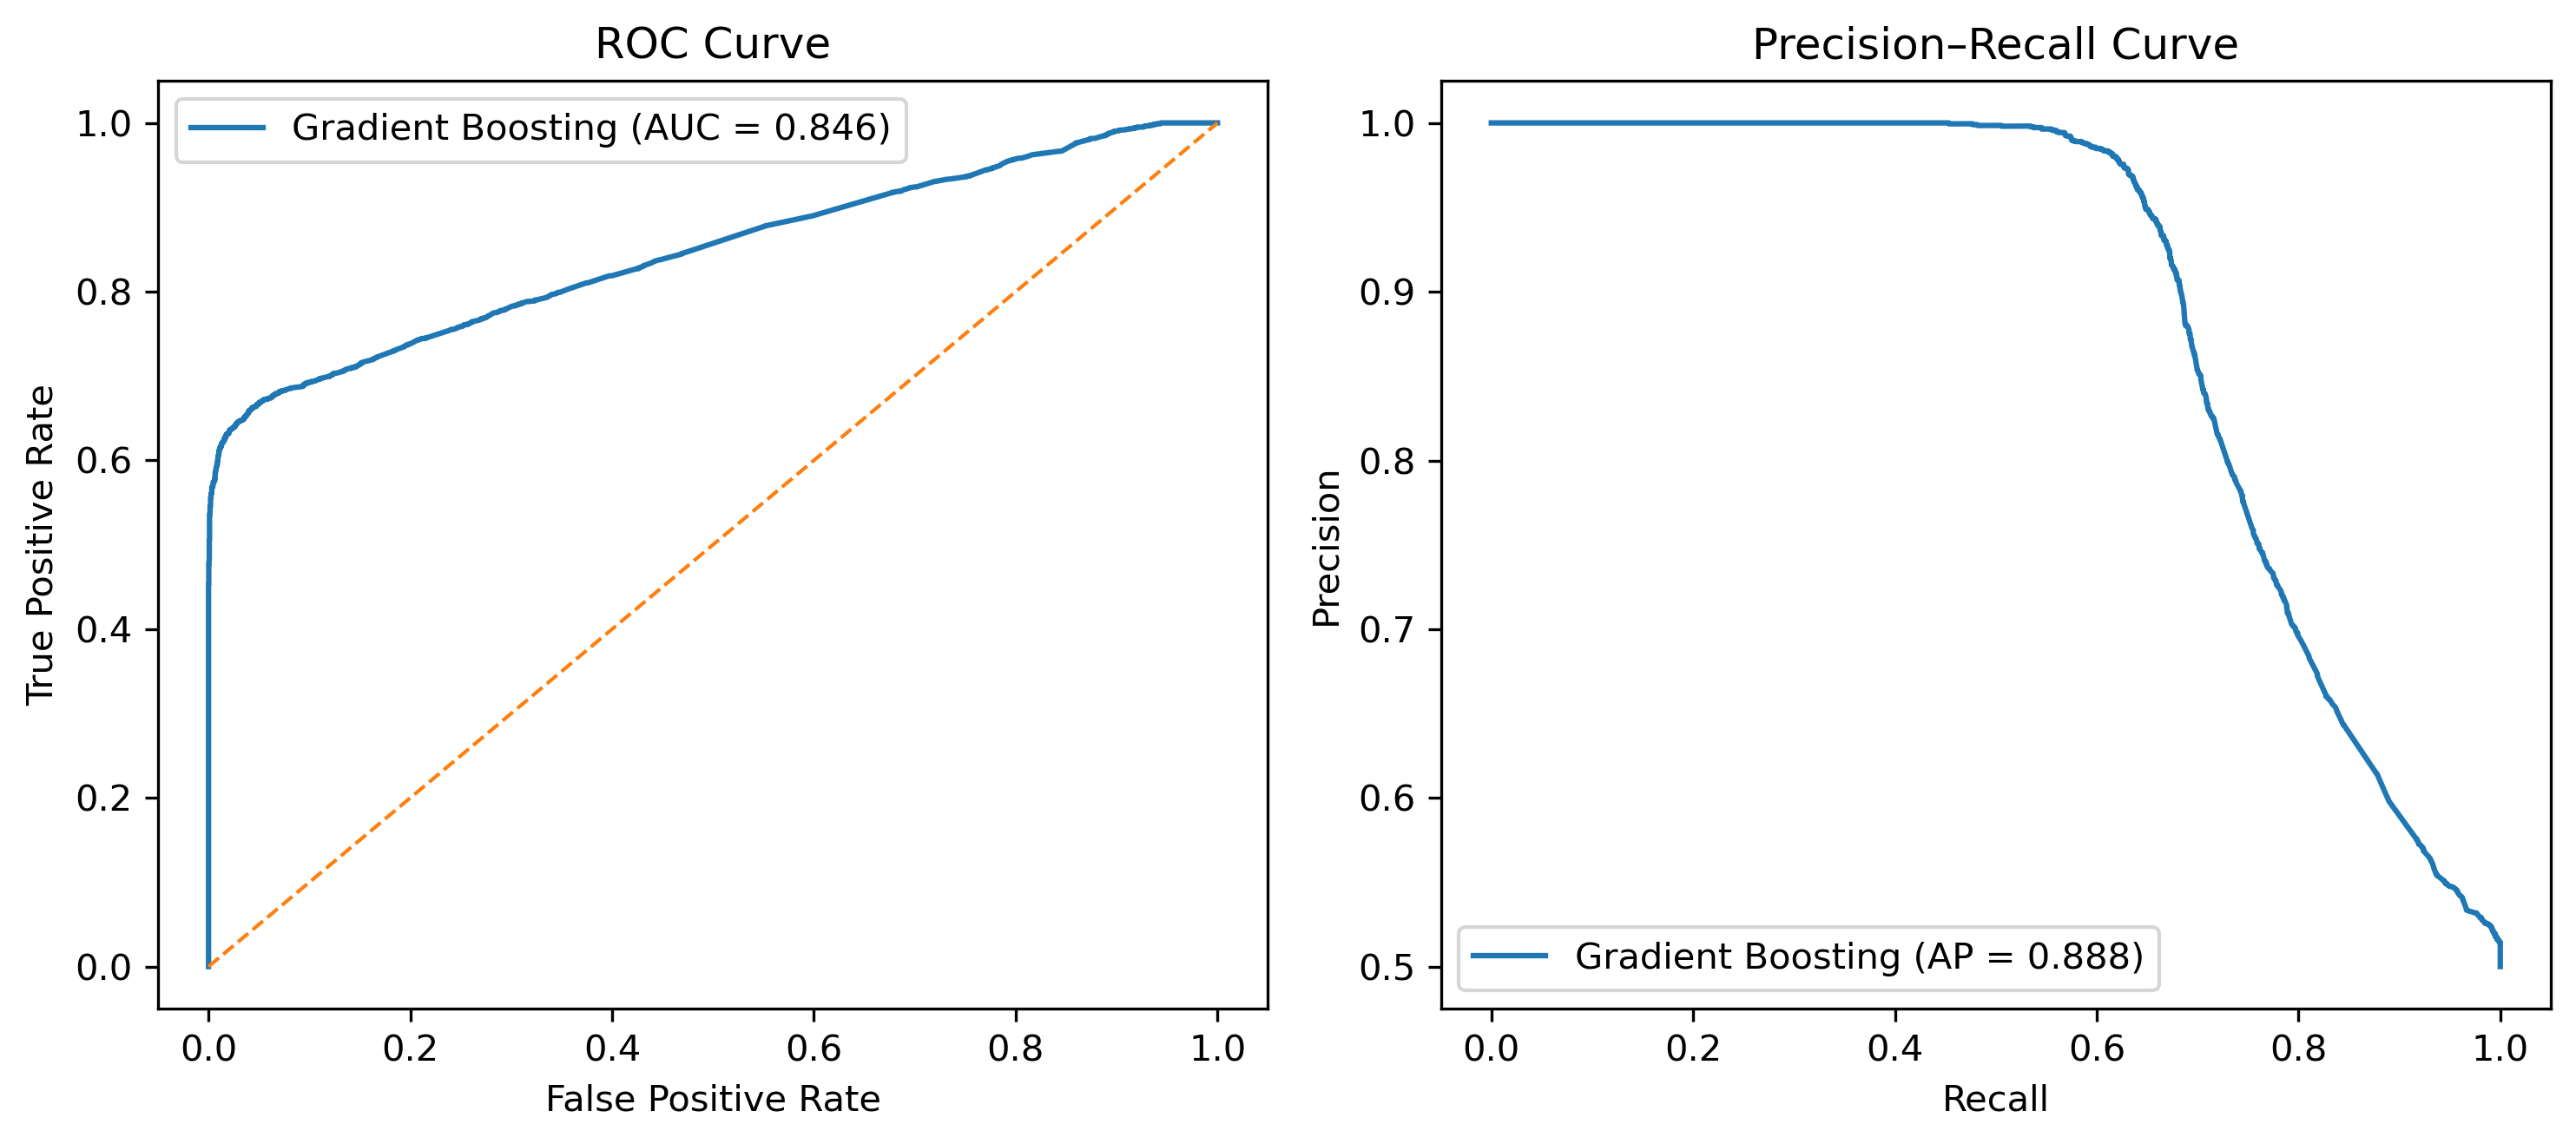
\includegraphics[width=0.8\linewidth]{figures/roc_pr_gradient_boosting.png}
\caption{ROC and precision--recall curves for the tuned Gradient Boosting classifier on the held-out test set.}
\label{fig:roc_pr_gradient_boosting}
\end{figure}

\section{Feature Importance}

\subsection{Permutation Importance of Individual Features}

To understand how the final classifier made predictions, feature importance was quantified using permutation importance for the tuned Gradient Boosting model.

As shown in Figure~\ref{fig:gradient_imp}, \texttt{total\_clipped\_bases} provides the strongest predictive signal, with an importance of 0.117. This is followed by \texttt{kmer\_js\_divergence} and \texttt{kmer\_cosine\_diff}, indicating that both clipping-based alignment irregularities and k-mer compositional shifts are central to the model’s decision-making process. In contrast, soft-clipping features contribute less strongly, while microhomology-related features such as \texttt{microhomology\_length} and \texttt{microhomology\_gc} provide minimal predictive value.

These results indicate that accurate detection of chimeric reads relies primarily on signals associated with breakpoint-related clipping patterns and abrupt compositional changes in sequence structure. By contrast, explicit microhomology features appear to add little information for this dataset.

\begin{figure}[H]
\centering

\includegraphics[width=0.6\linewidth]{figures/gradient_imp_pair.png}
\caption{Permutation-based feature importance for the tuned Gradient Boosting classifier.}
\label{fig:gradient_imp}
\end{figure}

\subsection{Feature Family Importance}

To evaluate broader predictive patterns, features were grouped into five families: SA\_structure, Clipping, Kmer\_jump, Micro\_homology, and Other.

For the tuned Gradient Boosting model, the Clipping family contributed the largest cumulative importance (0.134), followed by Kmer\_jump (0.096). The remaining families, namely SA\_structure, Micro\_homology, and Other, contributed only minimally. This pattern shows that the model draws most of its predictive power from alignment-based clipping signals and k-mer compositional changes, while explicit microhomology descriptors and other auxiliary alignment metrics play only a minor role.

Taken together, both feature-level and feature-family analyses indicate that Gradient Boosting relies primarily on breakpoint-associated clipping irregularities and shifts in local sequence composition to distinguish chimeric from clean reads. Supplementary permutation importance results across multiple classical models are provided in Appendix~\ref{app:supp_feature_importance}.

\begin{figure}[H]
\centering

\includegraphics[width=0.6\textwidth]{gradient_family_pair.png}
\caption{Aggregated feature family importance for the tuned Gradient Boosting classifier.}
\label{fig:gb_family}
\end{figure}

\section{Feature Selection}

Feature selection was performed to identify the smallest subset reaching 95\% cumulative importance. Three configurations were evaluated as references: the full Gradient Boosting model with all 24 features, a reduced model with the top-\(k\) features, and an ablation model excluding microhomology features, using the tuned Gradient Boosting classifier to assess feature contributions and overall classification performance.

\subsection{Cumulative Importance Curve}

The cumulative importance curve was computed using the tuned Gradient Boosting classifier. Figure~\ref{fig:cumulative_importance} shows that the importance rises steeply for the top-ranked features and then gradually plateaus, indicating that a relatively small number of predictors account for most of the model’s performance. A cumulative importance threshold of 95\% was reached at \(k = 4\) features: \texttt{total\_clipped\_bases}, \texttt{kmer\_js\_divergence}, \texttt{kmer\_cosine\_diff}, and \texttt{softclip\_left}.

\begin{figure}[H]
\centering
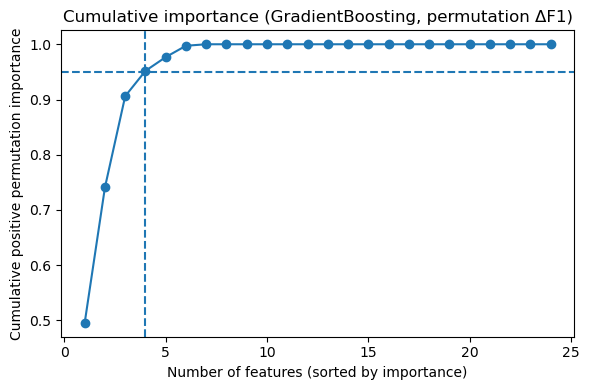
\includegraphics[width=0.6\textwidth]{figures/cumulative_gradient_pair.png}
\caption{Cumulative importance curve of features sorted by importance for the tuned Gradient Boosting classifier.}
\label{fig:cumulative_importance}
\end{figure}

\subsection{Performance Comparison Across Feature Sets}

Classification performance was compared across three feature sets using the tuned Gradient Boosting classifier. The full model, incorporating all 24 engineered features, achieved an F1-score of 0.7765 and a ROC--AUC of 0.8459. A reduced model using only the top four features (\texttt{total\_clipped\_bases}, \texttt{kmer\_js\_divergence}, \texttt{kmer\_cosine\_diff}, and \texttt{softclip\_left}) achieved nearly equivalent performance, with an F1-score of 0.7768 and a ROC--AUC of 0.8369. An ablation model excluding microhomology features (\texttt{microhomology\_length} and \texttt{microhomology\_gc}) also performed comparably, with an F1-score of 0.7761 and a ROC--AUC of 0.8444.

These findings indicate that clipping and k-mer features capture nearly all of the predictive signal used by the model, while microhomology features are largely redundant in this dataset.

\begin{table}[H]
\centering
\caption{Test set performance of feature set variants using the tuned Gradient Boosting classifier.}
\label{tab:gb_feature_sets}
\begin{tabular}{lrrr}
\toprule
Variant & No. of Features & Test F1 & ROC--AUC \\
\midrule
Full Gradient Boost & 24 & 0.7765 & 0.8459 \\
Selected (top-4) & 4 & 0.7768 & 0.8369 \\
No microhomology & 22 & 0.7761 & 0.8444 \\
\bottomrule
\end{tabular}
\end{table}

\begin{figure}[H]
\centering
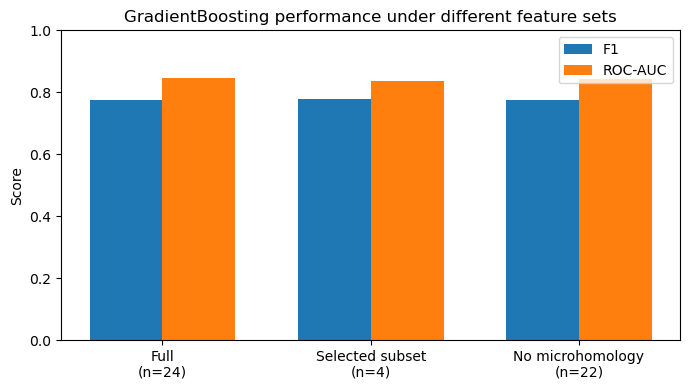
\includegraphics[width=0.6\textwidth]{figures/gradient_feature_sets_pair.png}
\caption{Comparison of F1 and ROC--AUC across feature set variants for the tuned Gradient Boosting classifier.}
\label{fig:gradient_boost_three_sets}
\end{figure}

\subsection{Interpretation and Final Feature Set Choice}

The full 24-feature Gradient Boosting model was retained as the primary configuration for the remainder of the study, while the four-feature subset is presented as a lightweight alternative. Clipping features reflect alignment junctions and mapping disruptions typical of chimeric reads, whereas k-mer divergence features capture abrupt changes in sequence composition across breakpoints. Microhomology features appear largely redundant, suggesting that their signal is either indirectly captured by clipping and k-mer descriptors or not strongly expressed in the simulation dataset.

\section{Convolutional Neural Network (CNN) Performance and Classification Results}

The CNN achieved strong and reasonably consistent performance across the five cross-validation folds, as summarized in Table~\ref{tab:cnn_cv_summary}. The mean validation loss across folds was 0.4444. The corresponding mean classification metrics were 0.8664 for accuracy, 0.8214 for precision, 0.9374 for recall, 0.8754 for F1-score, and 0.9359 for ROC--AUC. Across folds, F1-scores ranged from 0.8637 to 0.8898, while ROC--AUC values ranged from 0.9272 to 0.9467, indicating only modest variation in performance between validation splits.

\begin{table}[H]
\centering
\caption{Five-fold cross-validation performance of the CNN model.}
\label{tab:cnn_cv_summary}
\begin{tabular}{lrr}
\toprule
Metric & Mean & Std. Dev. \\
\midrule
Loss      & 0.4444 & 0.0308 \\
Accuracy  & 0.8664 & 0.0139 \\
Precision & 0.8214 & 0.0226 \\
Recall    & 0.9374 & 0.0083 \\
F1-score  & 0.8754 & 0.0110 \\
ROC--AUC  & 0.9359 & 0.0081 \\
\bottomrule
\end{tabular}
\end{table}

\begin{figure}[H]
\centering
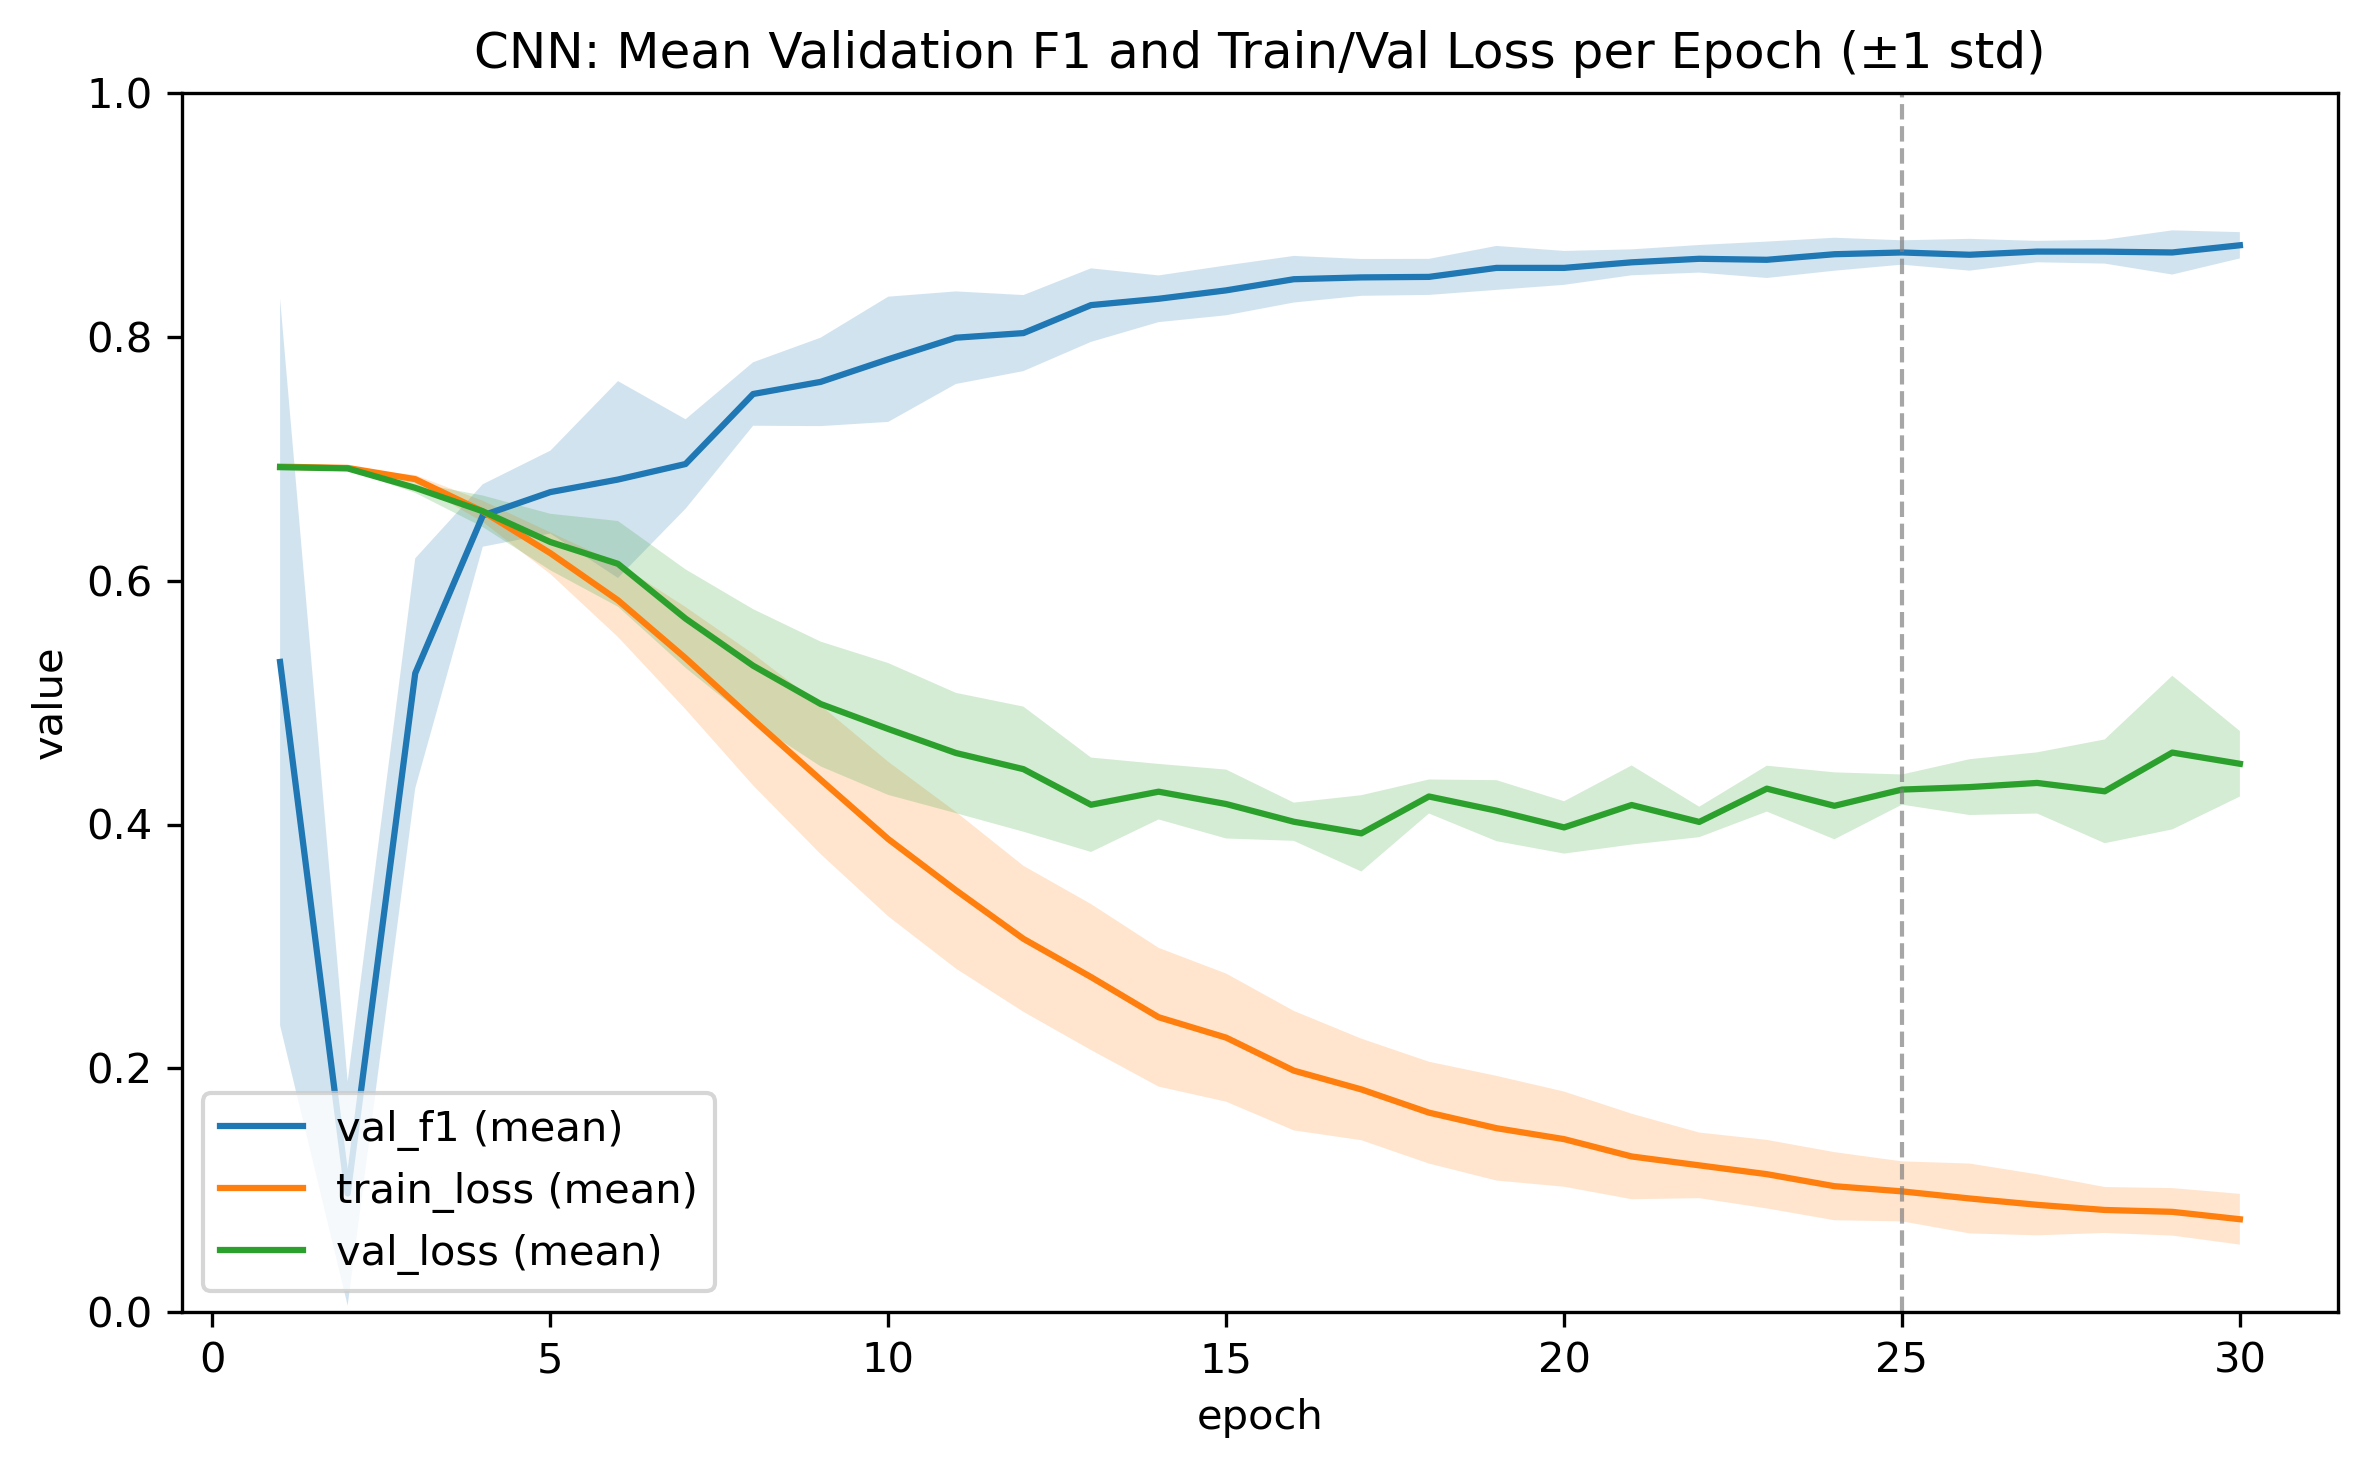
\includegraphics[width=\linewidth]{figures/cnn_cv_f1_loss_epoch25.png}
\caption{CNN training and validation loss and validation F1 across epochs.}
\label{fig:cnn_training}
\end{figure}

When evaluated on the held-out balanced test set, the final CNN achieved a test loss of 0.3034, accuracy of 0.9092, precision of 0.8724, recall of 0.9588, F1-score of 0.9135, and ROC--AUC of 0.9607, as shown in Table~\ref{tab:cnn_test_summary}. These results indicate that the model generalizes well beyond the validation folds and maintains strong classification performance on previously unseen data.

\begin{table}[H]
\centering
\caption{Held-out test performance of the CNN model.}
\label{tab:cnn_test_summary}
\begin{tabular}{lr}
\toprule
Metric & Value \\
\midrule
Loss      & 0.3034 \\
Accuracy  & 0.9092 \\
Precision & 0.8724 \\
Recall    & 0.9588 \\
F1-score  & 0.9135 \\
ROC--AUC  & 0.9607 \\
\bottomrule
\end{tabular}
\end{table}

As shown in Figure~\ref{fig:cnn_confusion}, the held-out test results indicate that the CNN is particularly effective at recovering chimeric reads, as reflected by its high recall. At the same time, its precision is lower than its recall, indicating that the model prioritizes sensitivity and accepts a moderate number of false-positive predictions in return. Nevertheless, the combination of a high F1-score and a ROC--AUC above 0.96 shows that the classifier still provides strong overall discrimination between clean and chimeric reads.

\begin{figure}[H]
\centering

\includegraphics[width=0.6\textwidth]{figures/cnn_confusion.png}
\caption{Confusion matrix of the CNN model on the held-out test set.}
\label{fig:cnn_confusion}
\end{figure}

\section{Recurrent Neural Network (RNN) Performance and Classification Results}

Across five cross-validation folds, the RNN-kmer BiGRU model achieved consistently high performance with low variability, as shown in Table~\ref{tab:rnn_cv_summary}. The mean cross-validation accuracy was 0.9303, mean precision was 0.9137, mean recall was 0.9505, mean F1-score was 0.9317, and mean ROC--AUC was 0.9734. Mean validation loss across folds was 0.3397. Individual fold F1-scores ranged from 0.9252 to 0.9386, while ROC--AUC ranged from 0.9672 to 0.9780, indicating only small variation across folds. Fold-level cross-validation results for the CNN and RNN-kmer BiGRU models are provided in Appendix~\ref{app:dl_fold_results}.

\begin{table}[H]
\centering
\caption{Five-fold cross-validation performance of the RNN-kmer BiGRU model.}
\label{tab:rnn_cv_summary}
\begin{tabular}{lrr}
\toprule
Metric & Mean & Std. Dev. \\
\midrule
Loss      & 0.3397 & 0.0619 \\
Accuracy  & 0.9303 & 0.0055 \\
Precision & 0.9137 & 0.0118 \\
Recall    & 0.9505 & 0.0094 \\
F1-score  & 0.9317 & 0.0051 \\
ROC--AUC  & 0.9734 & 0.0048 \\
\bottomrule
\end{tabular}
\end{table}

\begin{figure}[H]
\centering
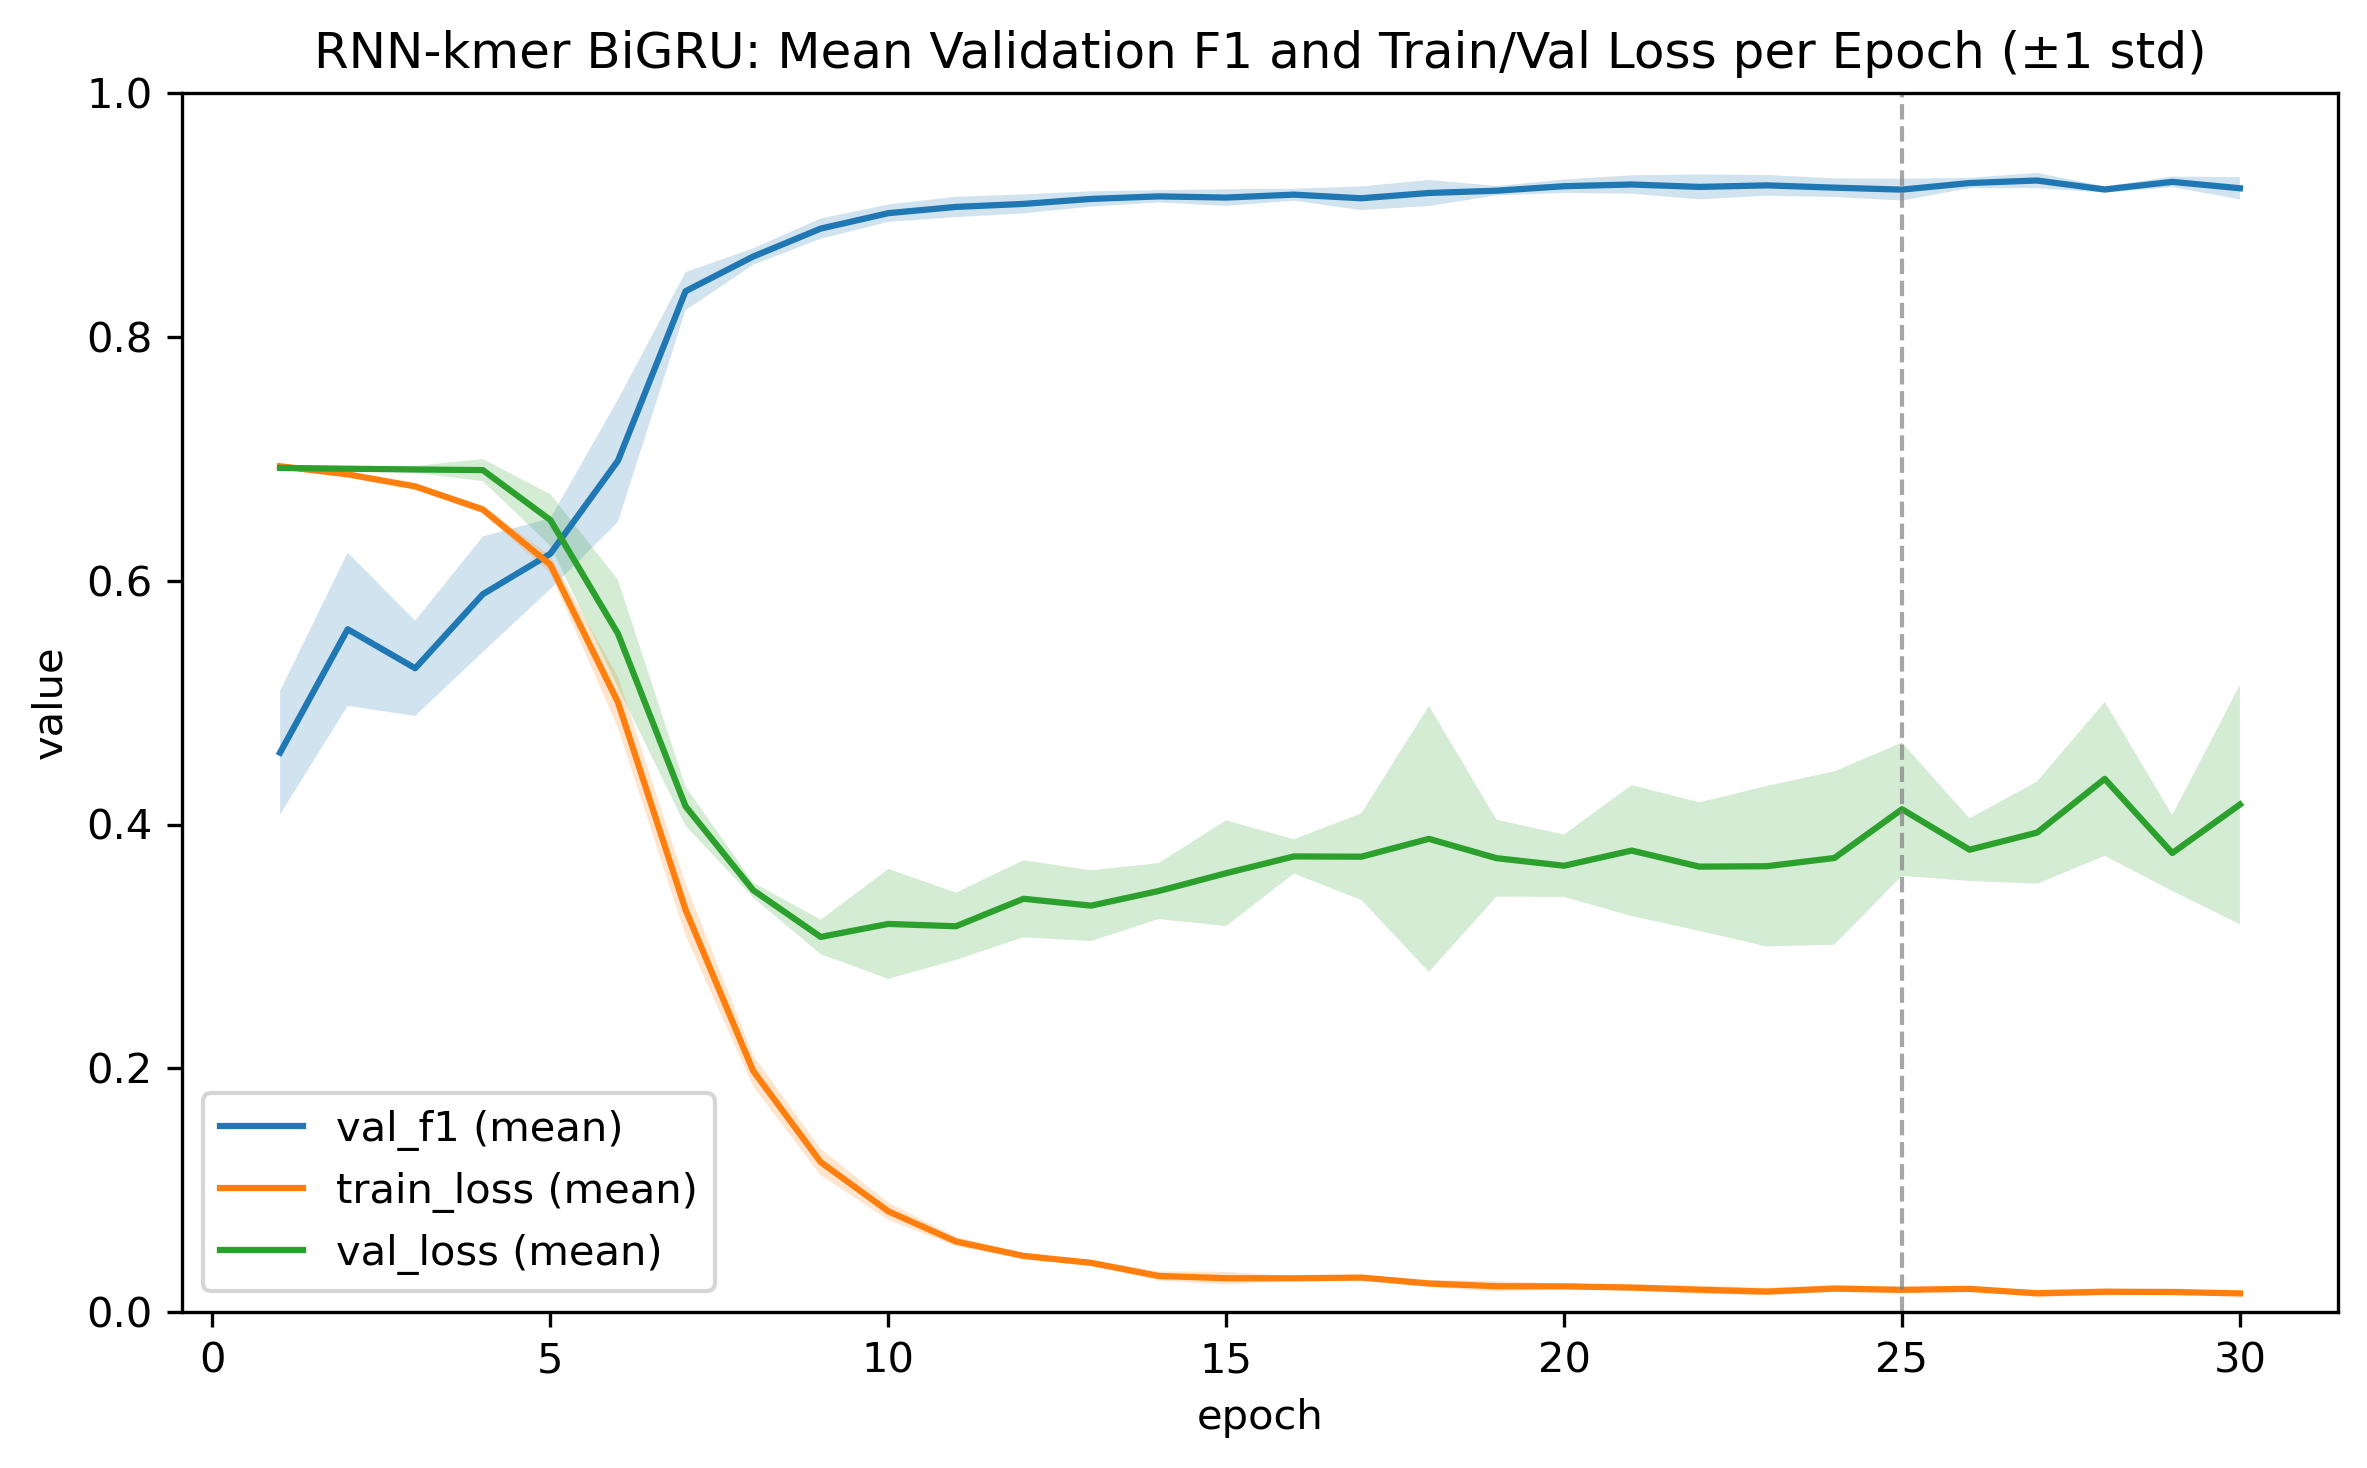
\includegraphics[width=\linewidth]{figures/rnn_cv_f1_loss_epoch25.png}
\caption{RNN-kmer BiGRU training and validation loss and validation F1 across epochs.}
\label{fig:rnn_training}
\end{figure}

On the held-out balanced test set (\(n = 8000\); 4000 clean and 4000 chimeric reads), the final RNN-kmer BiGRU model achieved a test loss of 0.2432, accuracy of 0.9516, precision of 0.9394, recall of 0.9655, F1-score of 0.9523, and ROC--AUC of 0.9849, as summarized in Table~\ref{tab:rnn_test_summary}. These values exceed those of both the tuned Gradient Boosting classifier and the CNN.

\begin{table}[H]
\centering
\caption{Held-out test performance of the RNN-kmer BiGRU model.}
\label{tab:rnn_test_summary}
\begin{tabular}{lr}
\toprule
Metric & Value \\
\midrule
Loss      & 0.2432 \\
Accuracy  & 0.9516 \\
Precision & 0.9394 \\
Recall    & 0.9655 \\
F1-score  & 0.9523 \\
ROC--AUC  & 0.9849 \\
\bottomrule
\end{tabular}
\end{table}

Figure~\ref{fig:rnn_confusion} shows that the model correctly classified 3751 of 4000 clean reads and 3862 of 4000 chimeric reads. Only 249 clean reads were incorrectly labeled as chimeric, while 138 chimeric reads were misclassified as clean.

\begin{figure}[H]
\centering

\includegraphics[width=0.6\textwidth]{figures/rnn_confusion.png}
\caption{Confusion matrix of the RNN-kmer BiGRU model on the held-out test set.}
\label{fig:rnn_confusion}
\end{figure}

\subsection{External Assembly Testing}

\subsubsection{3200 Paired-end Reads}

At the minimum read depth (3200), assembly outcomes depended strongly on how many reads were retained after filtering. At 5\% chimeras, all filters resolved minor branching by reducing the graph from 2 nodes (unfiltered) to 1 node. However, at higher chimera rates, filtering effects diverged. The CNN filter produced fragmentation at 15--50\% chimeras (2 nodes), consistent with aggressive read removal, where CNN retained only 48.78--75.19\% of reads. BiGRU maintained a 1-node graph at 10--15\% chimeras while retaining 75.56--78.94\% of reads, but at 50\% chimeras the graph fragmented into 8 nodes after retention dropped to 44.59\%. In contrast, GB maintained a 1-node graph across these conditions by retaining more reads (77.88--95.22\%).

\subsubsection{10K Paired-end Reads}

At 10K reads and 5--15\% chimeras, all assemblies produced a clean 1-node graph, indicating that filtering mainly affected read retention rather than assembly structure. At 50\% chimeras, the unfiltered graph branched into 3 nodes. Filtering reduced this complexity, with GB, CNN, and BiGRU each producing 2 nodes. GB retained 78.94\% of reads, CNN retained 49.47\%, and BiGRU retained 44.68\%. The residual nodes under all three filters suggest that even after filtering, some ambiguous reads remained that were sufficient to sustain minor branches, although graph complexity was still reduced relative to the unfiltered condition.

\subsubsection{20K Paired-end Reads}

At 20K reads, unfiltered assemblies showed increased branching at 10--15\% chimeras (3 nodes) and extreme fragmentation at 50\% (966 nodes). All filters restored contiguity. BiGRU produced a 1-node graph at 5--15\% chimeras while retaining 75.13--83.84\% of reads, and reduced the 50\% chimera graph to 2 nodes with 44.85\% retention. At this highest chimera level, CNN produced the simplest graph (1 node) with 49.89\% retention, whereas GB produced 3 nodes while retaining substantially more reads (78.49\%). These results indicate that at higher coverage, more stringent filtering reduced graph complexity relative to GB. In the 50\% chimera condition, CNN yielded a more simplified graph than BiGRU, as BiGRU still produced 2 nodes despite retaining a smaller proportion of reads.

Across read depths, GB consistently retained the highest proportion of reads and generally preserved contiguous assemblies, making it the most reliable at low depth (3200). BiGRU showed an intermediate behaviour between GB and CNN. It retained fewer reads than GB and, under high chimera burden, reduced graph complexity more than GB, although not as effectively as CNN. At the minimum depth, BiGRU became risky at high chimera percentage, where retention dropped to 44.59\% and the assembly fragmented into 8 nodes, as shown in Figure~\ref{fig:3200_50_nodes}. Overall, assembly outcomes depended on both read depth and chimera percentage. At higher coverage, stronger filtering could reduce graph complexity, but the extent of simplification varied across models: CNN achieved the strongest simplification at high chimera percentage, whereas BiGRU showed only partial simplification under the same condition, as illustrated in Figure~\ref{fig:20k_50_nodes}. At minimum coverage, stronger filtering could reduce read support sufficiently to split the assembly into multiple nodes. In some unfiltered conditions, Bandage still showed a single-node graph. This does not imply the absence of chimeric reads; rather, SPAdes outputs a simplified assembly graph after trimming tips and removing erroneous, including chimeric, connections. If chimeric reads do not generate an alternative path with sufficient support to persist through simplification, the assembly collapses to one dominant segment and appears as a single node in Bandage \cite{Bankevich2012SPAdes,Antipov2016SPAdesHybrid,Wick2015Bandage}. Supplementary assembly graph figures for all evaluated external testing conditions are provided in Appendix~\ref{app:assembly_figures}. Complete external assembly testing results across all evaluated conditions are provided in Appendix~\ref{app:assembly_tables}.

\begin{figure}[htbp]
\centering
\caption{Assembly graphs for 20K paired-end reads at 50\% chimera proportion.}
\label{fig:20k_50_nodes}

\begin{subfigure}[b]{0.48\textwidth}
\centering
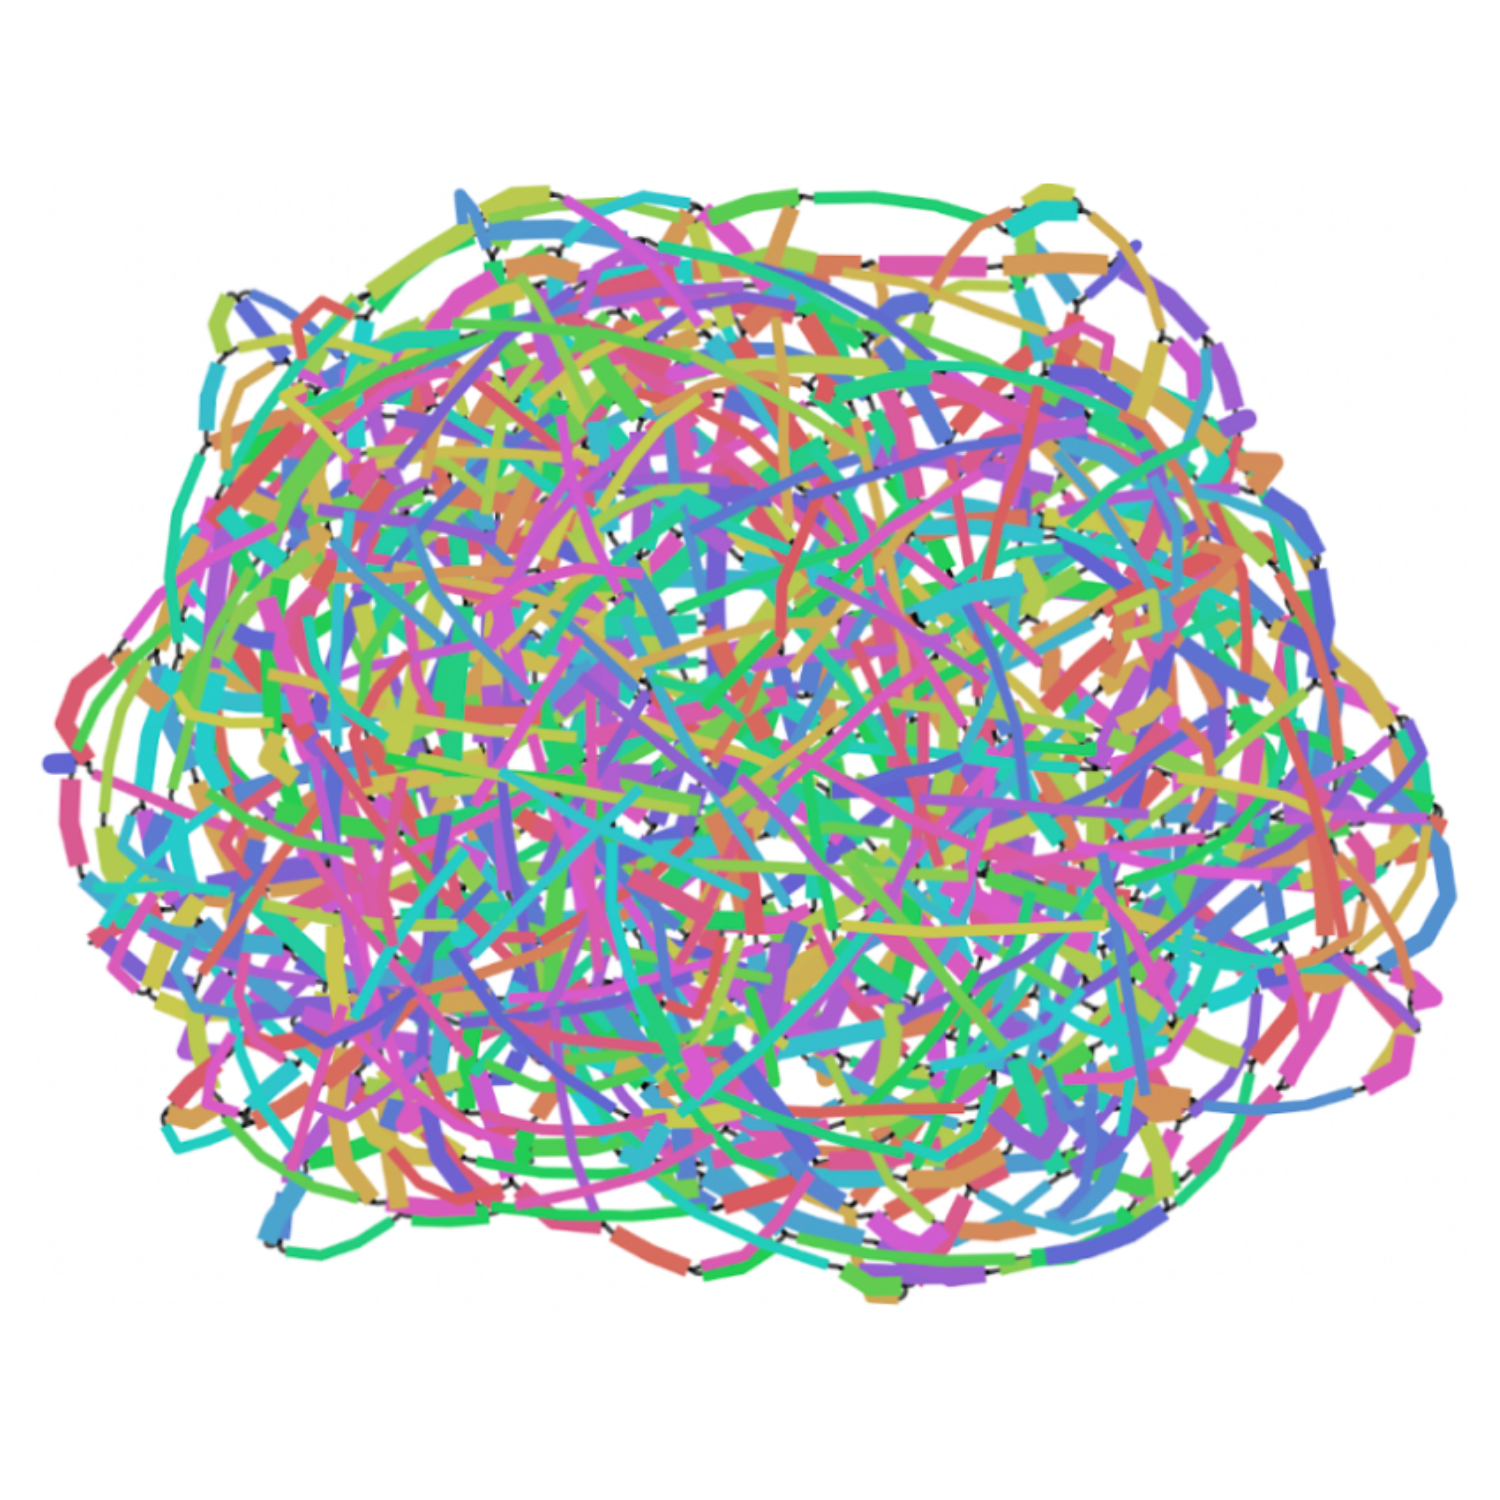
\includegraphics[width=\linewidth]{figures/20knodes_unfiltered.png}
\caption{Unfiltered}
\label{fig:20k_50_unfiltered}
\end{subfigure}
\hfill
\begin{subfigure}[b]{0.48\textwidth}
\centering
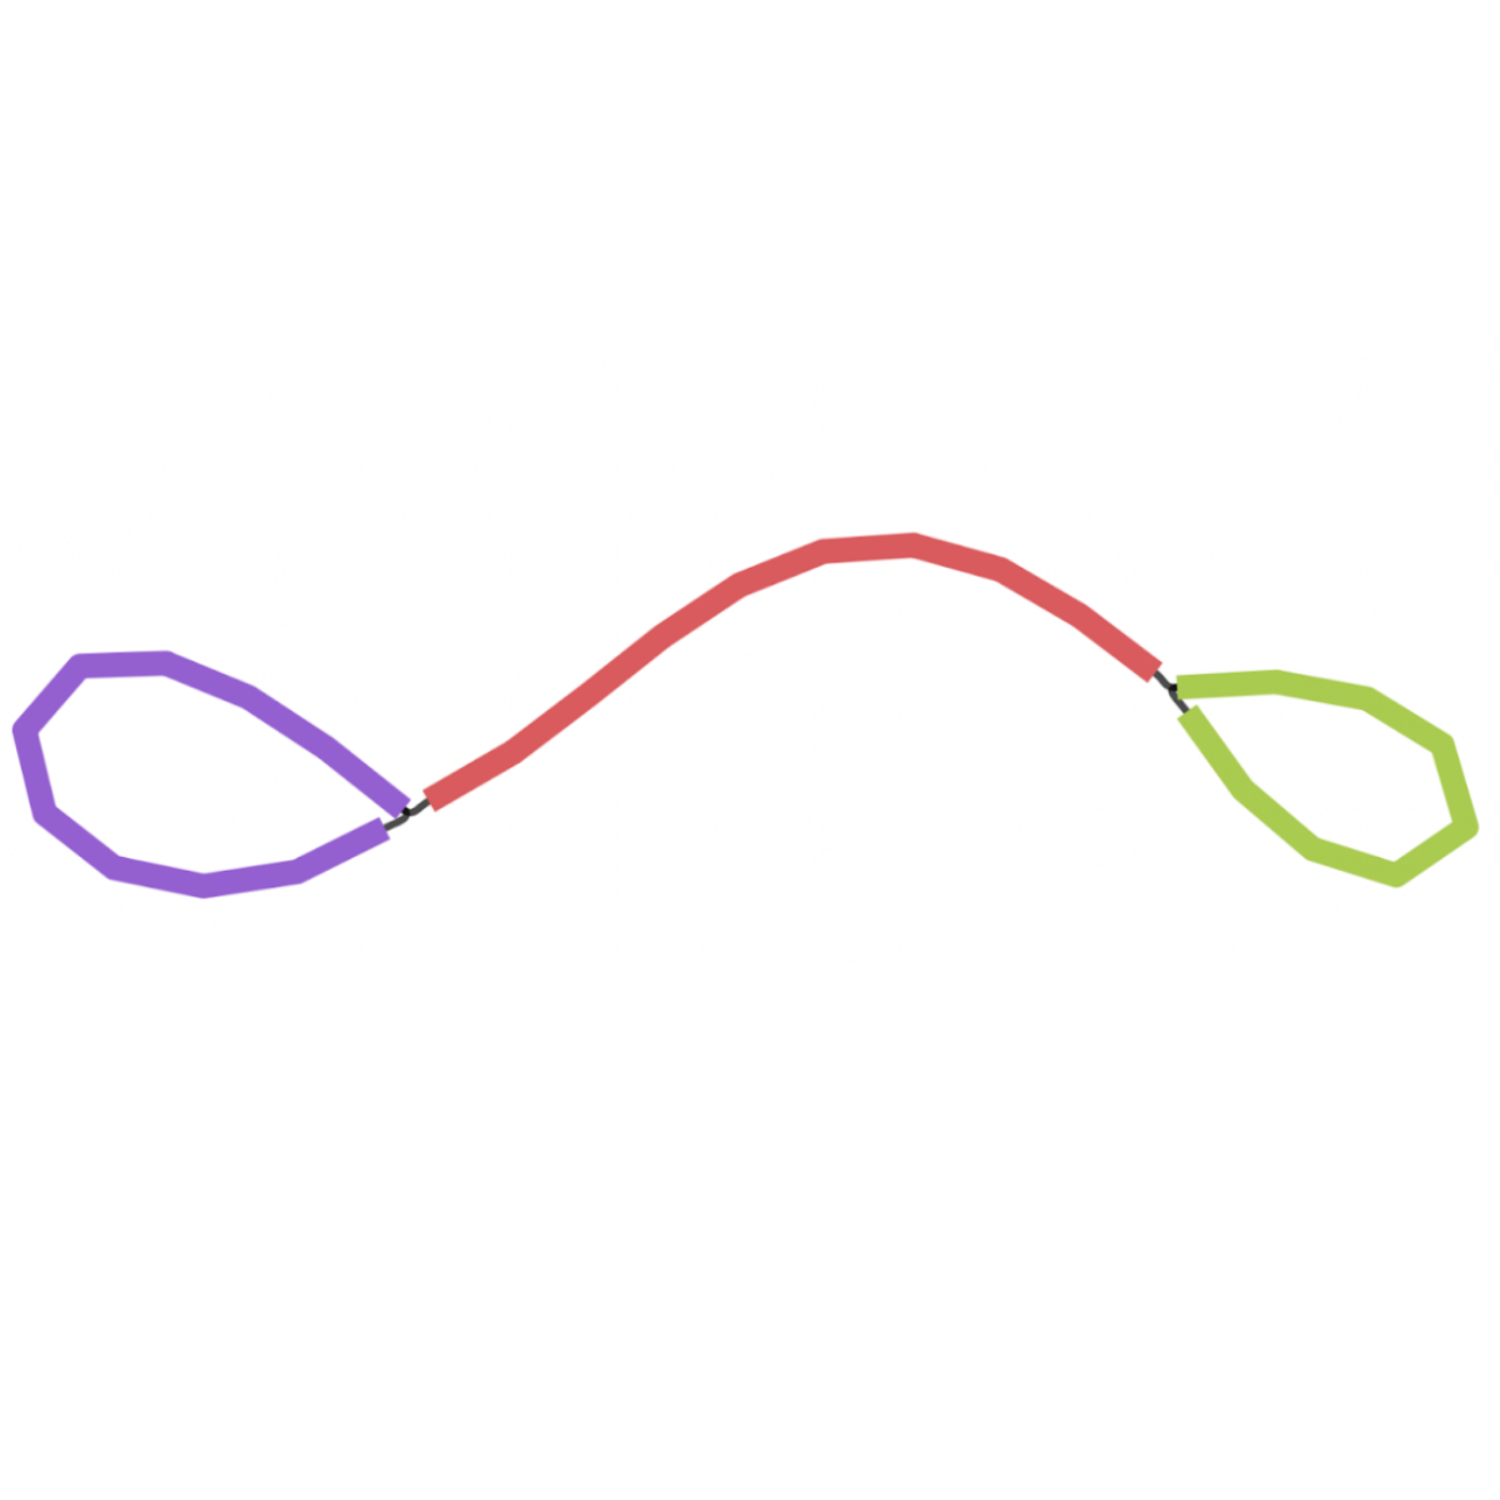
\includegraphics[width=\linewidth]{figures/20knodes_gb.png}
\caption{GB}
\label{fig:20k_50_gb}
\end{subfigure}

\vspace{0.5em}

\begin{subfigure}[b]{0.48\textwidth}
\centering
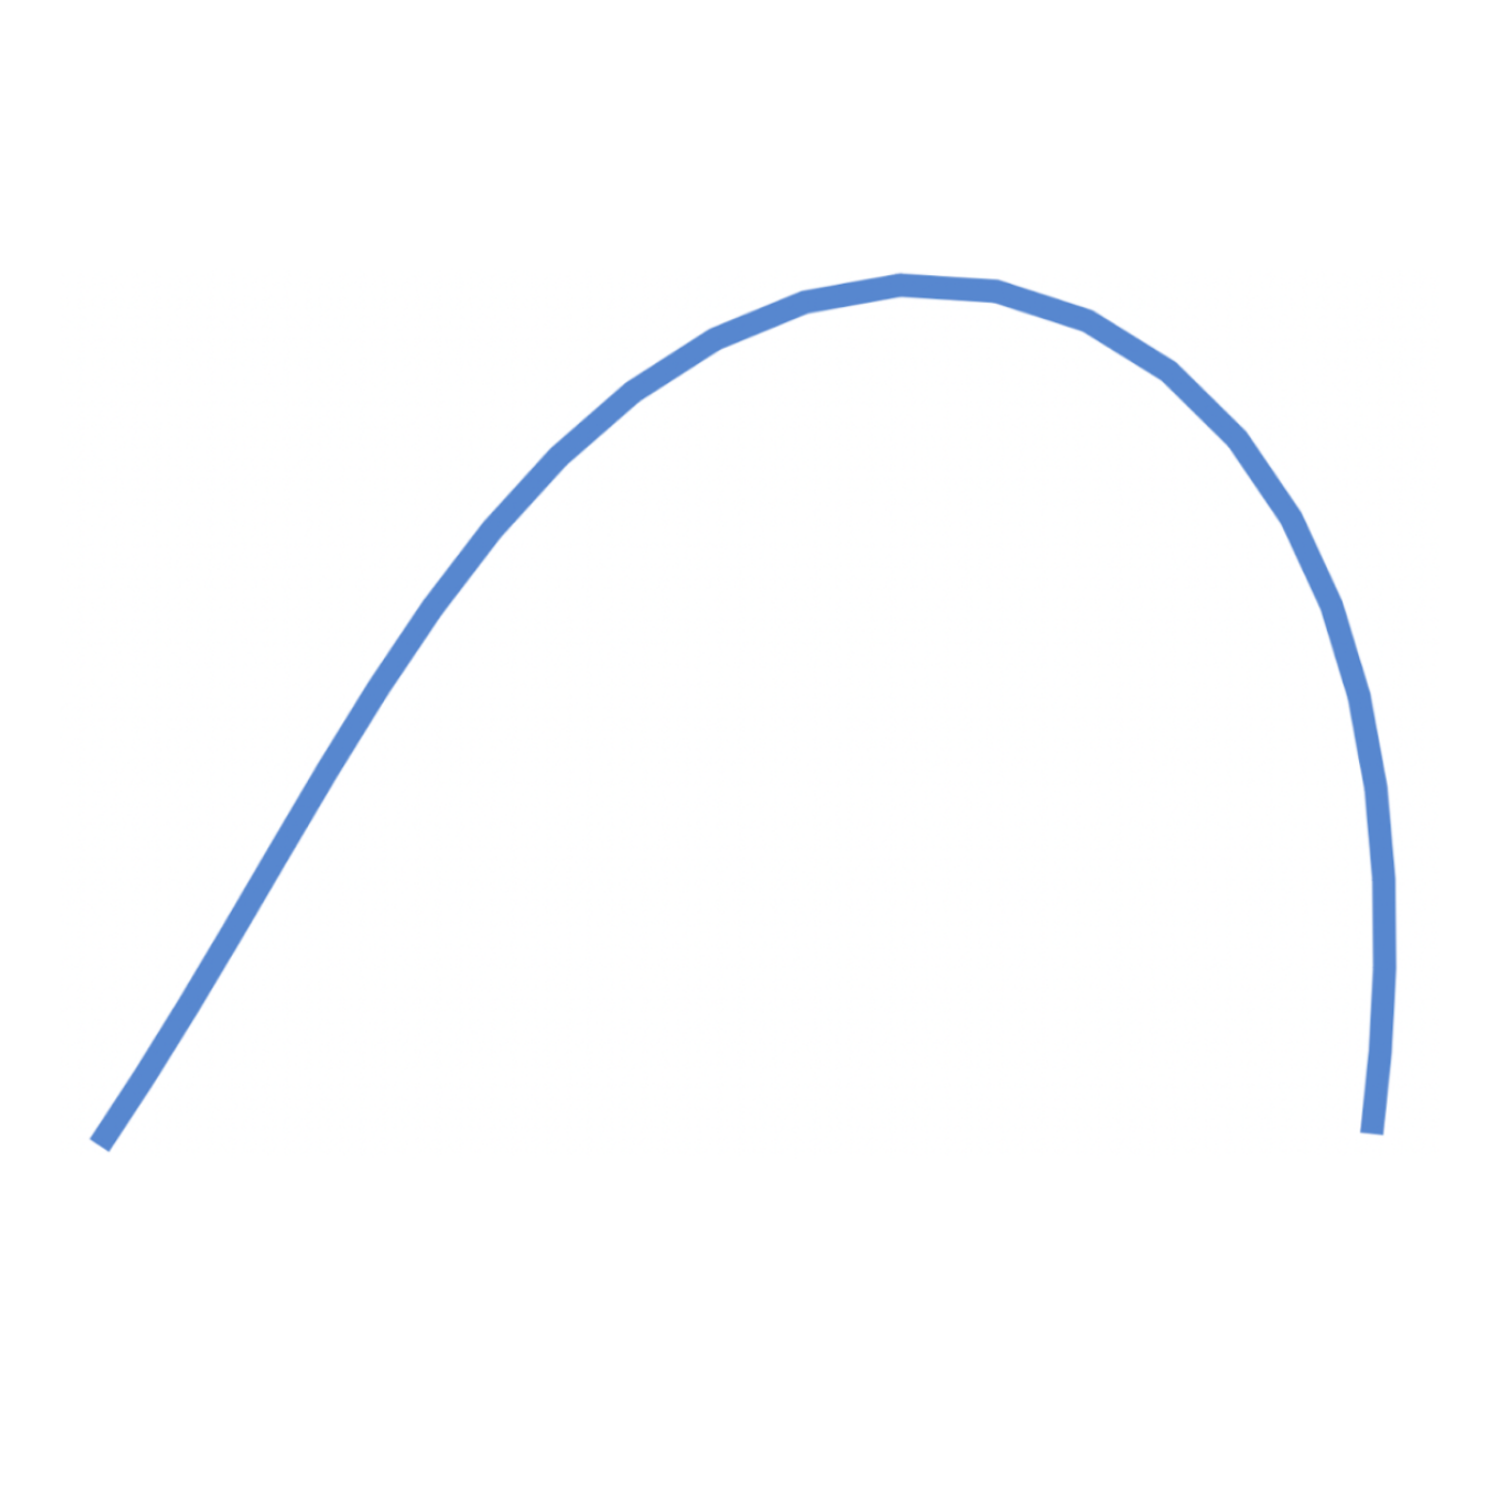
\includegraphics[width=\linewidth]{figures/20knodes_cnn.png}
\caption{CNN}
\label{fig:20k_50_cnn}
\end{subfigure}
\hfill
\begin{subfigure}[b]{0.48\textwidth}
\centering
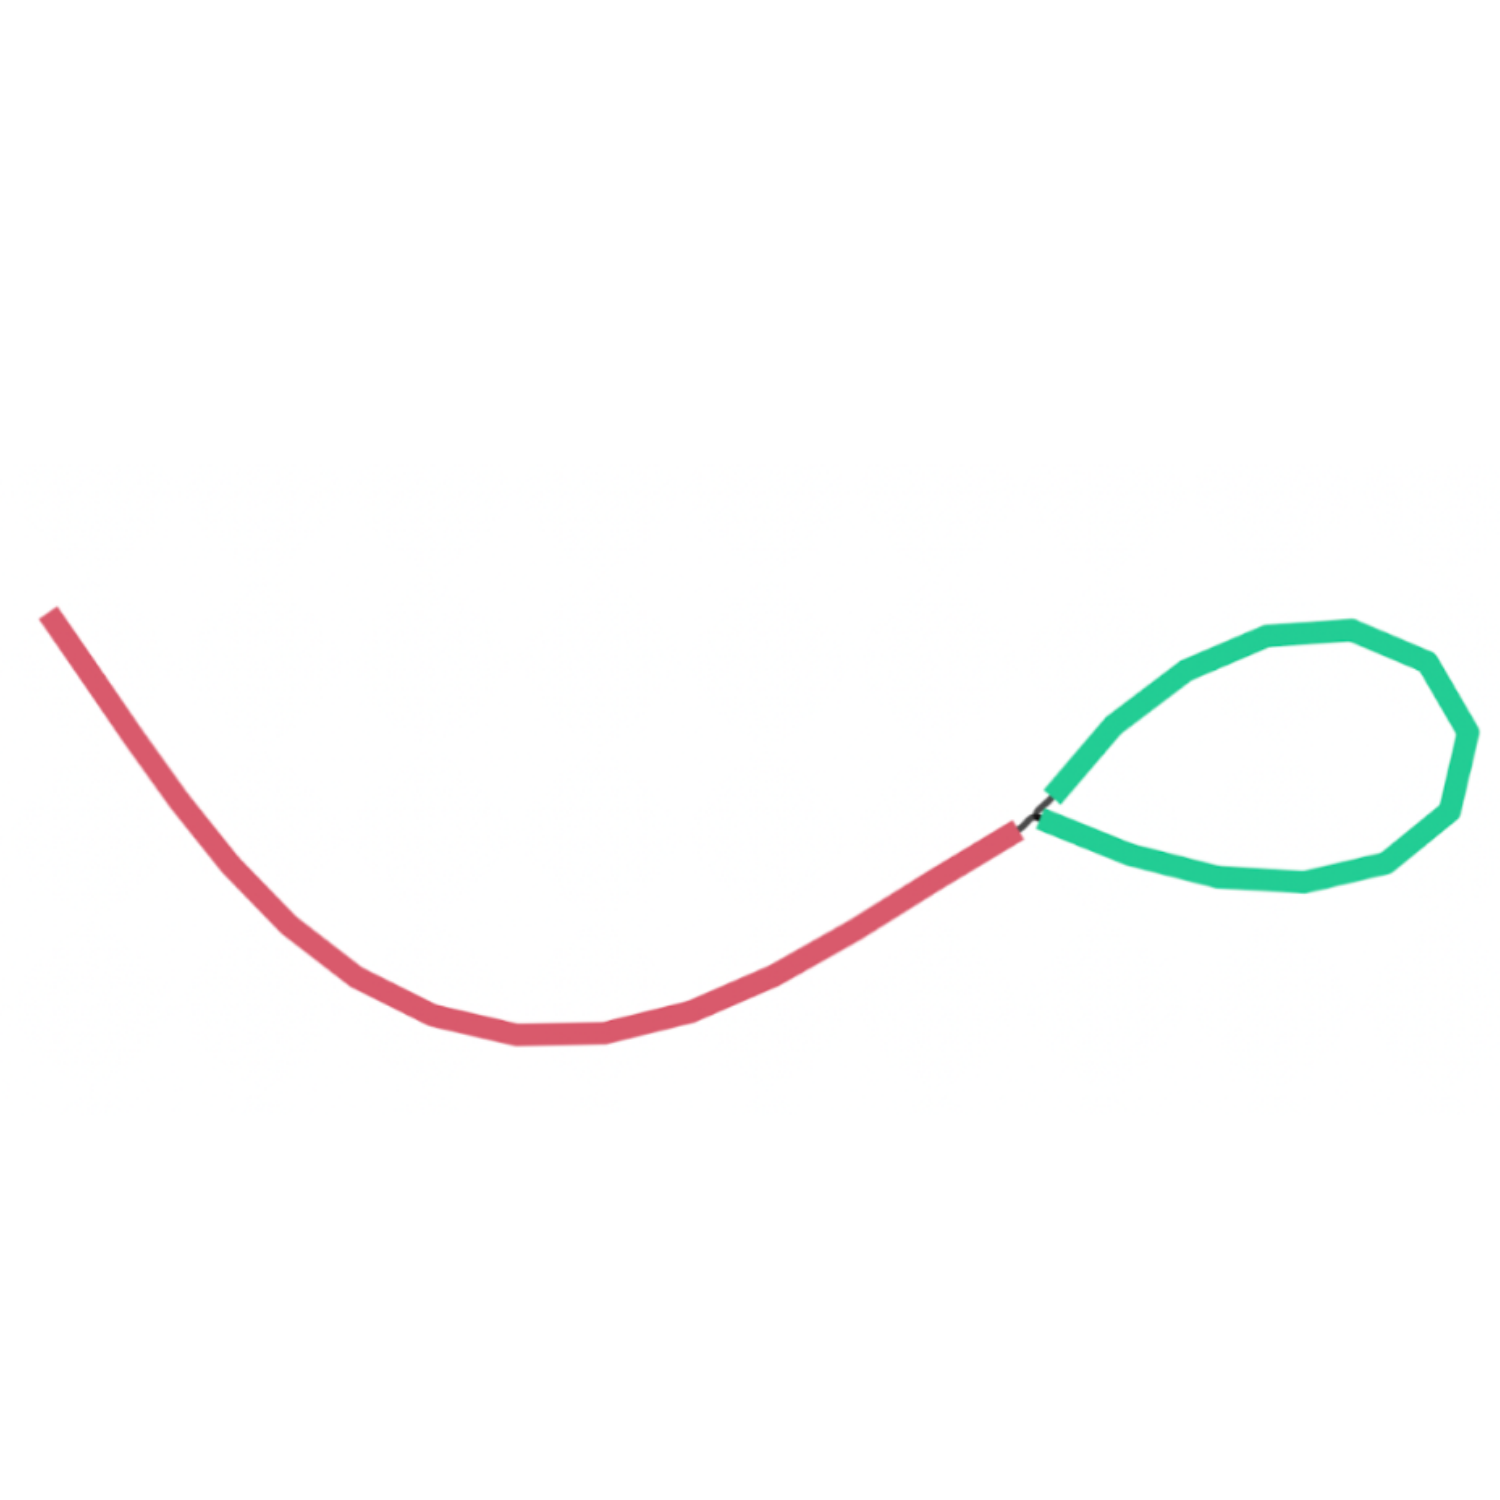
\includegraphics[width=\linewidth]{figures/20knodes_rnn.png}
\caption{BiGRU}
\label{fig:20k_50_bigru}
\end{subfigure}
\end{figure}

\begin{figure}[htbp]
\centering
\caption{Assembly graphs for 3200 paired-end reads at 50\% chimera proportion.}
\label{fig:3200_50_nodes}

\begin{subfigure}[b]{0.48\textwidth}
\centering

\includegraphics[width=\linewidth]{figures/3200nodes_unfiltered.png}
\caption{Unfiltered}
\label{fig:3200_50_unfiltered}
\end{subfigure}
\hfill
\begin{subfigure}[b]{0.48\textwidth}
\centering
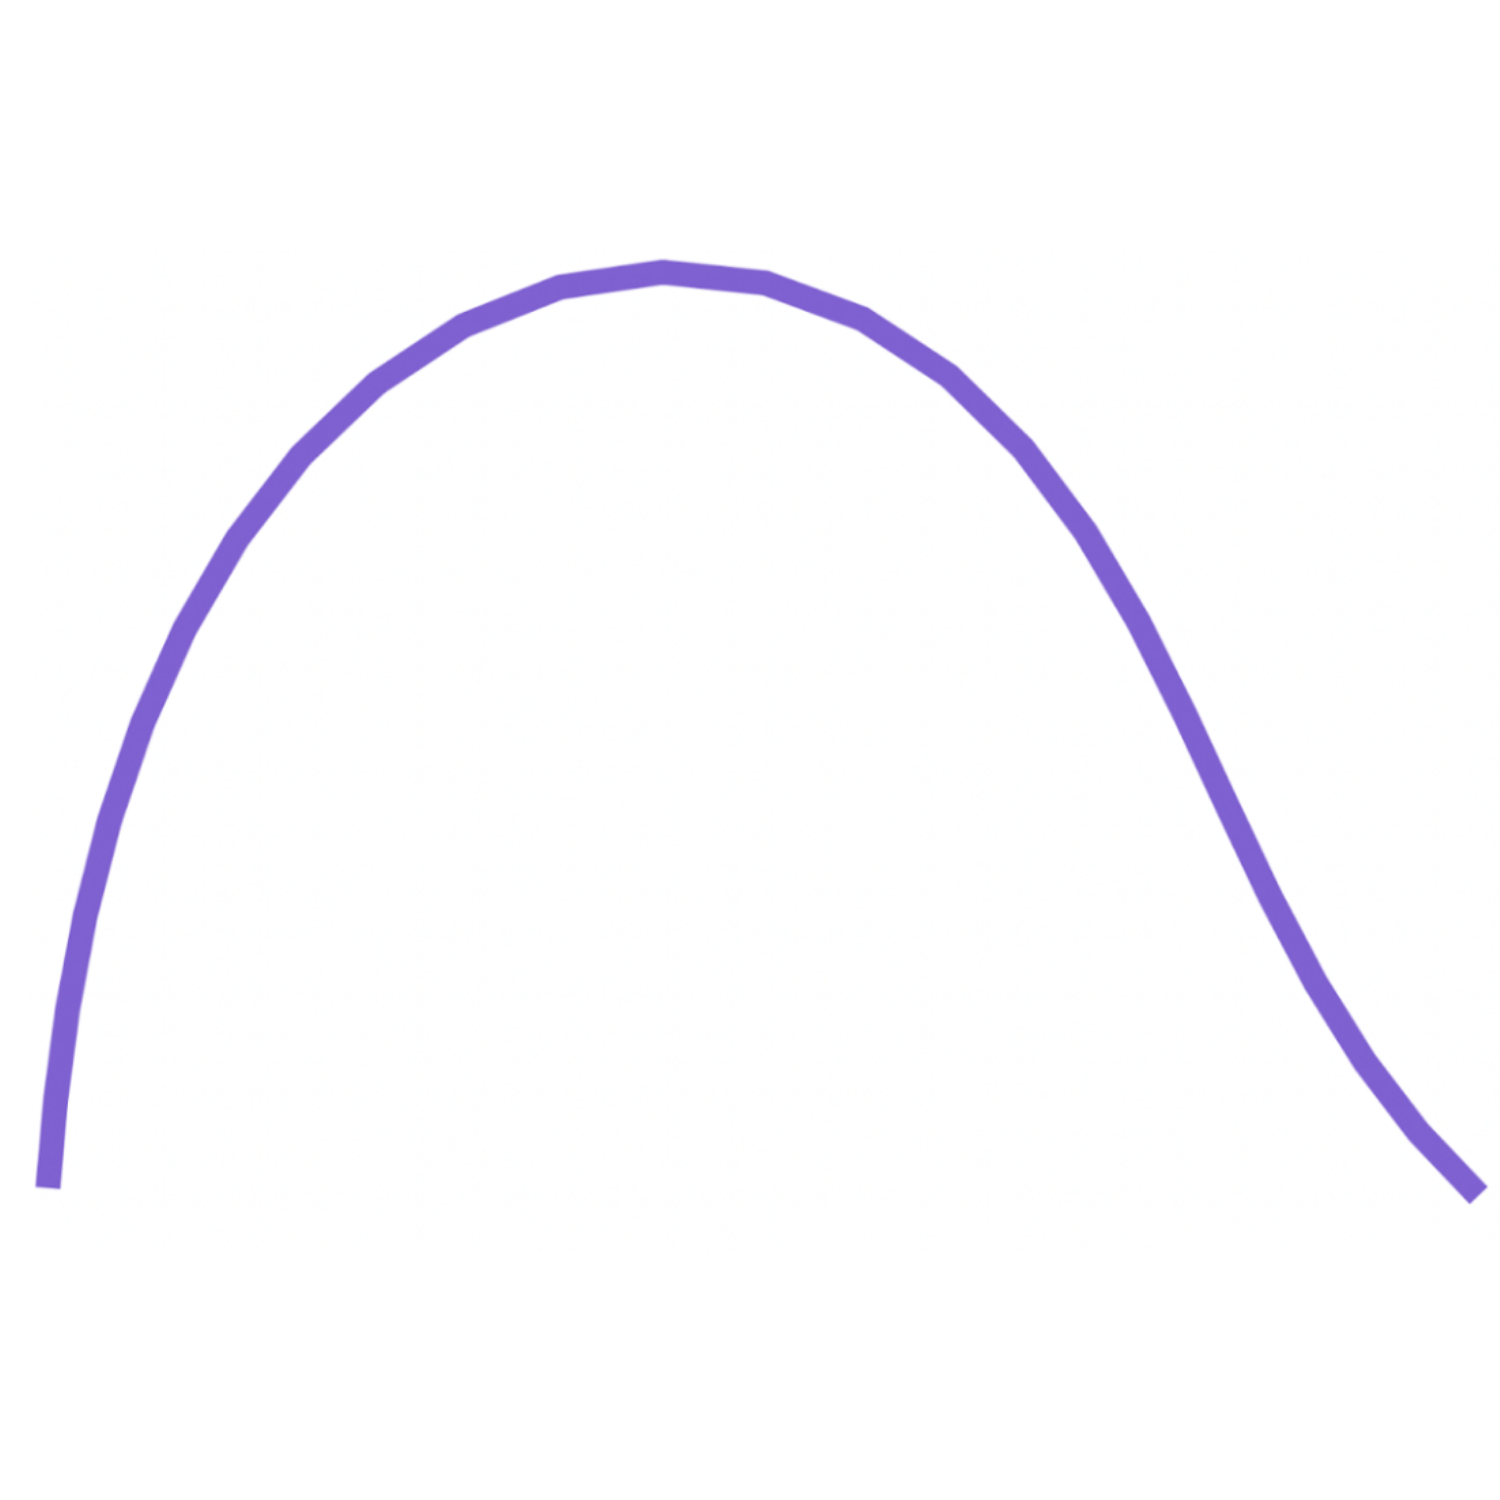
\includegraphics[width=\linewidth]{figures/3200nodes_gb.png}
\caption{GB}
\label{fig:3200_50_gb}
\end{subfigure}

\vspace{0.5em}

\begin{subfigure}[b]{0.48\textwidth}
\centering

\includegraphics[width=\linewidth]{figures/3200nodes_cnn.png}
\caption{CNN}
\label{fig:3200_50_cnn}
\end{subfigure}
\hfill
\begin{subfigure}[b]{0.48\textwidth}
\centering
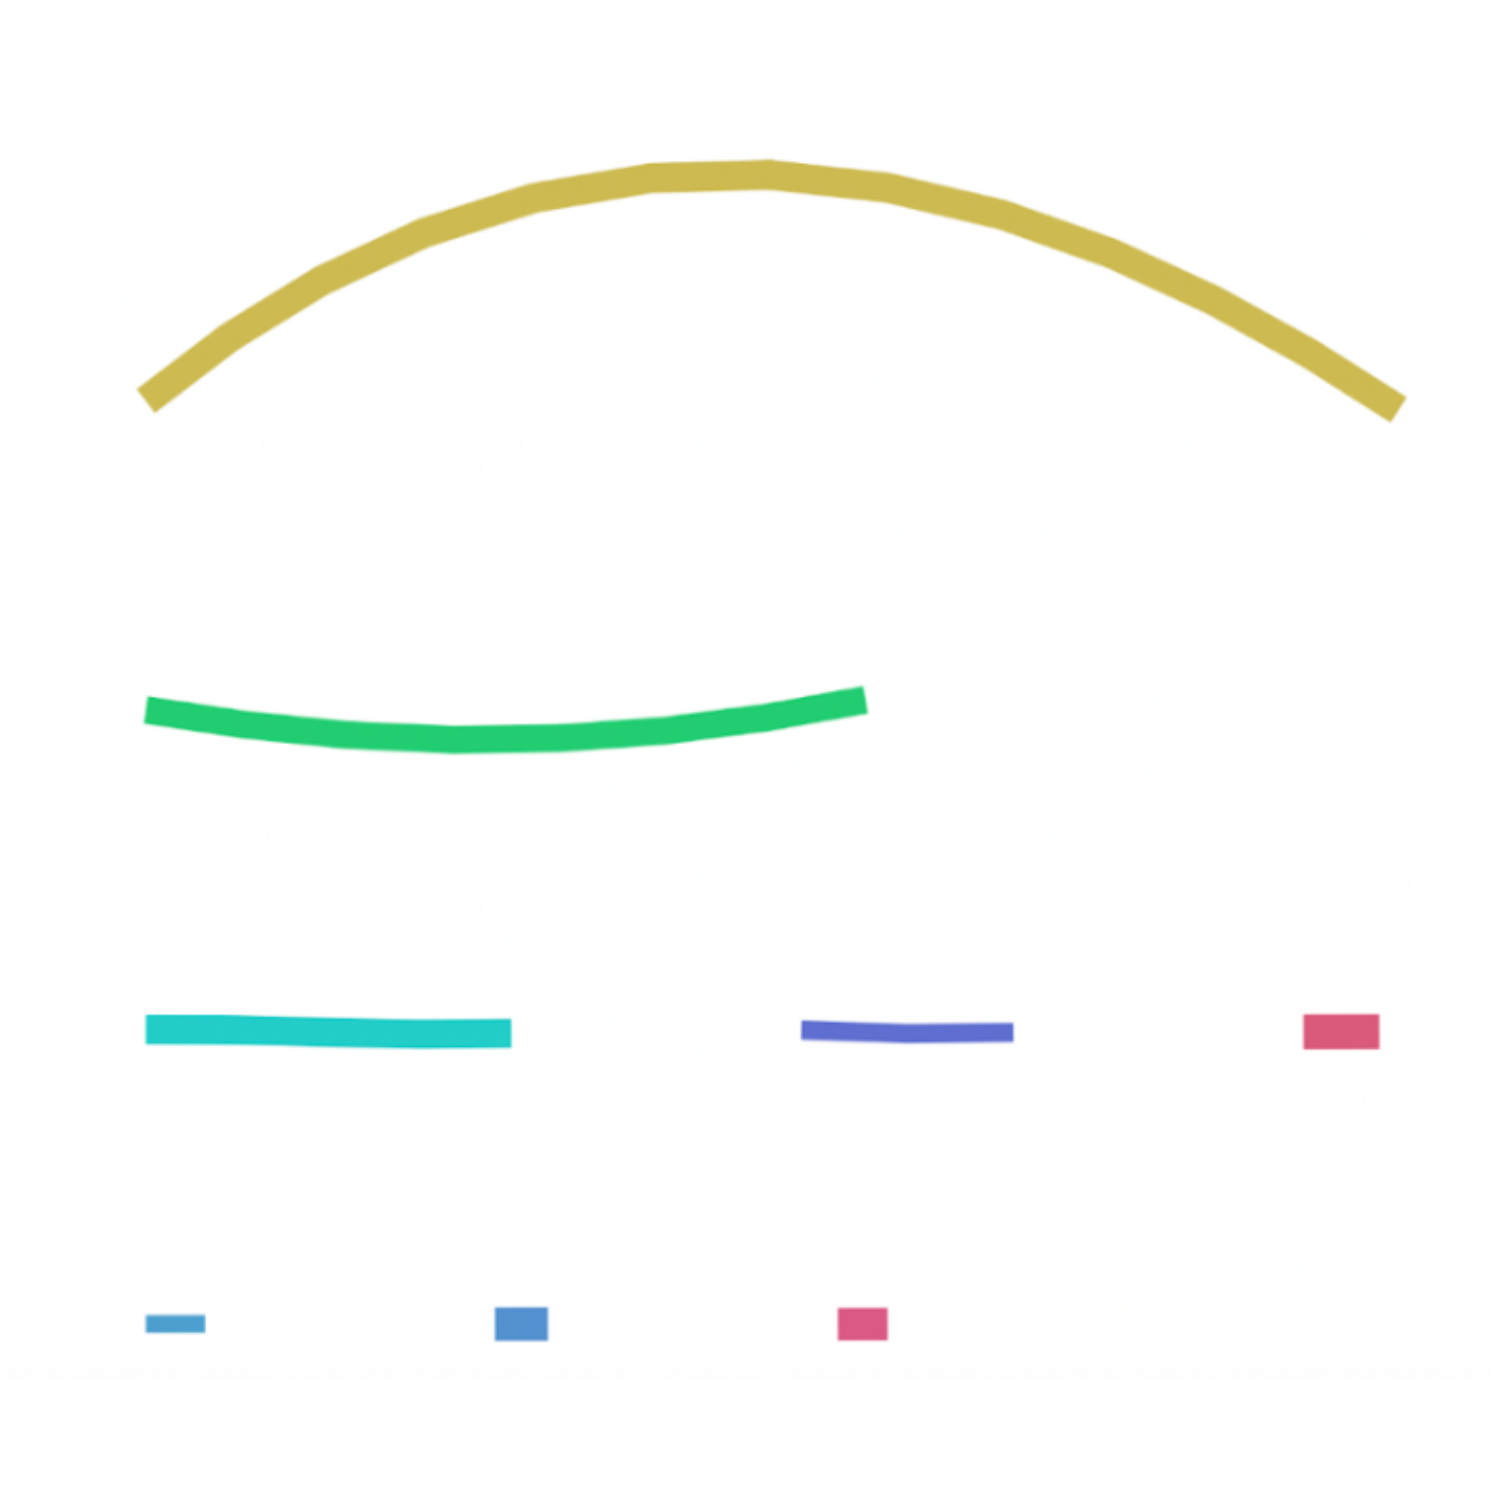
\includegraphics[width=\linewidth]{figures/3200nodes_rnn.png}
\caption{BiGRU}
\label{fig:3200_50_bigru}
\end{subfigure}
\end{figure}

\subsection{Comparison Across Models}

Direct comparison of the three best-performing approaches, shown in Table~\ref{tab:gb_cnn_rnn_compare} and Figure~\ref{fig:gb_cnn_rnn_compare}, shows a clear ranking. All models were trained and evaluated in the Kaggle environment. The tuned Gradient Boosting model achieved an F1-score of 0.7765 and ROC--AUC of 0.8459 with the shortest elapsed time of 0.50 minutes. The CNN improved substantially to an F1-score of 0.9135 and ROC--AUC of 0.9607, with an elapsed time of 1.39 minutes. The RNN-kmer BiGRU surpassed both in predictive performance, reaching an F1-score of 0.9523 and ROC--AUC of 0.9849, but required the longest elapsed time at 5.51 minutes.

\begin{table}[H]
\centering
\small
\caption{Comparison of held-out test performance and runtime across the top-performing models.}
\label{tab:gb_cnn_rnn_compare}
\begin{tabular}{lrrrrrr}
\toprule
Model & Accuracy & Precision & Recall & F1-score & ROC--AUC & Runtime (min) \\
\midrule
Gradient Boosting (tuned) & 0.8091 & 0.9368 & 0.6630 & 0.7765 & 0.8459 & 0.50 \\
CNN1D                     & 0.9093 & 0.8724 & 0.9588 & 0.9135 & 0.9607 & 1.39 \\
RNN-kmer BiGRU            & 0.9516 & 0.9394 & 0.9655 & 0.9523 & 0.9849 & 5.51 \\
\bottomrule
\end{tabular}
\end{table}

\begin{figure}[H]
\centering

\includegraphics[width=0.75\linewidth]{figures/gb_cnn_rnn_compare.png}
\caption{Comparison of held-out test F1 and ROC--AUC for Gradient Boosting, CNN, and RNN models.}
\label{fig:gb_cnn_rnn_compare}
\end{figure}